\documentclass[12pt, a4paper, oneside]{Thesis} % Paper size, default font size and one-sided paper
\usepackage{wrapfig}
\usepackage{lscape}
\usepackage{rotating}
\usepackage{graphicx}
\usepackage{caption}
\usepackage{amsmath}


\usepackage{lineno,hyperref}
\modulolinenumbers[5]


\usepackage{amssymb}
\usepackage{graphicx}
\usepackage{array}
\usepackage{float}
\usepackage{placeins}
\usepackage{stackengine}
\usepackage{url}
\usepackage{numprint}
\usepackage{caption}

\usepackage{booktabs}  
\usepackage{siunitx}
%\usepackage[showframe=false]{geometry}
\usepackage{subfigure}
\usepackage[square,numbers]{natbib}
\nprounddigits{3}
\newcolumntype{P}[1]{>{\centering\arraybackslash}p{#1}}
\newcolumntype{M}[1]{>{\centering\arraybackslash}m{#1}}

\setstackEOL{\#}
\setstackgap{L}{12pt}


%\usepackage{subcaption} %incompatible with subfig
\graphicspath{{Pictures/}} % Specifies the directory where pictures are stored
\usepackage{natbib} % Use the natbib reference package - read up on this to edit the reference style; if you want text (e.g. Smith et al., 2012) for the in-text references (instead of numbers), remove 'numbers' v

\hypersetup{urlcolor=black, colorlinks=false} % Colors hyperlinks in blue - change to black if annoyingv`	

\thesistitle{Automated Detection of Mind Wandering state from Electroencephalogram data using different Machine Learning techniques}
\supervisor{Professor Debasis Samanta}
\degree{Master of Technology}
\degreemajor{Computer Science and Engineering}
\authors{Sachin Kumar}
\rollno{15CS30025}
\university{Indian Institute of Technology Kharagpur}
\department{Department of Computer Science and Engineering}
\unisite{http://iitkgp.ac.in}
\depsite{http://cse.iitkgp.ac.in}
\placeshrt{Kharagpur}
\placelng{Kharagpur - 721302, India}
\datesub{June 2, 2020}
\datesig{June 2, 2020}
\semsub{Spring Semester, 2019-20}
% \keywords{Steel Structure}
\coursecd{Project-II(CS57004) }

\title{\ttitle} % Defines the thesis title - don't touch this
\begin{document}
%\makeatletter
%\renewcommand*{\NAT@nmfmt}[1]{\textsc{#1}}
%\makeatother

% prints author names as small caps


\frontmatter % Use roman page numbering style (i, ii, iii, iv...) for the pre-content pages

\setstretch{1.6} % Line spacing of 1.6 (double line spacing)

% Define the page headers using the FancyHdr package and set up for one-sided printing
\fancyhead{} % Clears all page headers and footers
\rhead{\thepage} % Sets the right side header to show the page number
\lhead{} % Clears the left side page header

%\pagestyle{fancy} % Finally, use the "fancy" page style to implement the FancyHdr headers

\newcommand{\HRule}{\rule{\linewidth}{0.5mm}} % New command to make the lines in the title page

% PDF meta-data
\hypersetup{pdftitle={\ttitle}}
\hypersetup{pdfsubject=\subjectname}
\hypersetup{pdfauthor=\authornames}
\hypersetup{pdfkeywords=\keywordnames}

%----------------------------------------------------------------------------------------
%	TITLE PAGE
%----------------------------------------------------------------------------------------
\maketitle
%\titlepg % Add a gap in the Contents, for aesthetics

\clearpage % Start a new page

%----------------------------------------------------------------------------------------
%	DECLARATION PAGE
%	Your institution may give you a different text to place here
%----------------------------------------------------------------------------------------


\Declaration% Add a gap in the Contents, for aesthetics


%----------------------------------------------------------------------------------------
%	CERTIFICATE PAGE
%----------------------------------------------------------------------------------------

\addtotoc{Certificate} % Add the "Abstract" page entry to the Contents

\certificate{\addtocontents{toc}{} % Add a gap in the Contents, for aesthetics

\clearpage % Start a new page

%----------------------------------------------------------------------------------------
%	ABSTRACT PAGE
%----------------------------------------------------------------------------------------

\addtotoc{Abstract} % Add the "Abstract" page entry to the Contents

\abstract{\addtocontents{toc}{} % Add a gap in the Contents, for aesthetics

\justifying
Mind Wandering (MW) is the recurrent occurrence in which our mind gets disengaged from the immediate task and focuses on internal trains of thought. There are some specific brain regions which are more active during the MW than alertness state,the brain network made by combination of these regions is called default mode network (DMN).In my MTP-I project, I have identified brain region that constitute the DMN using EEG signals only.Mind Wandering,which is quite common in our daily life,can be effectively detected using EEG signals.There are few attempts that has been made to predict MW state using machine learning analysis of EEG data however, there are still chances of further improvement in term of detection accuracy. Therefore, in this project we proposed a set of sequential steps based on data processing and machine learning to detect MW over data collected by EEG. In our study, we extracted a number of features from 64 internal EEG channels.The prediction accuracy of the proposed method is higher than the other researches under this field using ML only.On extracted features, we have applied different ML  classification techniques; we compared the results obtain from these techniques.It was found that the Random Forest classifier produces the highest detection accuracy in this context.

% The default mode network (DMN), which represents areas that are more active during times of rest compared to times of cognitive activity. The DMN is routinely identified with functional magnetic resonance imaging (fMRI) or positron emission tomography (PET). However, both of these methods limits the domain of the groups of patients that can be examined. We show that the DMN can also be identified by electroencephalography (EEG). Instructing subjects to alternate between self-referential memory recall and focusing on their breathing induces a spatial pattern of spectral band power modulation in the $\theta$ - and $\alpha$-band (4–16 Hz) that is consistent with the DMN pattern observed with PET and fMRI. Since
% EEG is a portable, cheap, and safe technology, our work enables the characterization of DMN alterations in patient groups that are difficult to study with fMRI or PET. 
    

}

\clearpage % Start a new page



%----------------------------------------------------------------------------------------
%	ACKNOWLEDGEMENTS
%----------------------------------------------------------------------------------------

\setstretch{1.3} % Reset the line-spacing to 1.3 for body text (if it has changed)

\acknowledgements{\addtocontents{toc}{}%\vspace{1em}} % Add a gap in the Contents, for aesthetics

I would first like to thank my supervisor Professor Debasis Samanta of the Computer Science and Engineering Department at Indian Institute of technology,Kharagpur. The door to Asso. Prof. D. Samanta office was always open whenever I ran into a trouble spot or had a question about my project or writing. He consistently allowed this paper to be my own work, but steered me in the right the direction whenever he thought I needed it.

I  would  also  like  to  thank  all  the  Panels  who  were  involved  in  the  validation survey for this M.tech project.Without their passionate participation and input, the validation survey could not have been successfully conducted.

I would also like to thank Mr. Subrata Pain (PhD scholar )for providing me with unfailing support and continuous encouragement throughout my project.

}
\clearpage % Start a new page

%----------------------------------------------------------------------------------------
%	LIST OF CONTENTS/FIGURES/TABLES PAGES
%----------------------------------------------------------------------------------------

\pagestyle{fancy} % The page style headers have been "empty" all this time, now use the "fancy" headers as defined before to bring them back

\lhead{\emph{Contents}} % Set the left side page header to "Contents"
\tableofcontents % Write out the Table of Contents

\lhead{\emph{List of Figures}} % Set the left side page header to "List of Figures"
\listoffigures % Write out the List of Figures

\lhead{\emph{List of Tables}} 
\listoftables
% \lhead{\emph{List of Tables}} % Set the left side page header to "List of Tables"
% \listoftables % Write out the List of Tables

%----------------------------------------------------------------------------------------
%	ABBREVIATIONS
%----------------------------------------------------------------------------------------

\clearpage % Start a new page

\setstretch{1.5} % Set the line spacing to 1.5, this makes the following tables easier to read

\lhead{\emph{Abbreviations}} % Set the left side page header to "Abbreviations"
\listofsymbols{ll} % Include a list of Abbreviations (a table of two columns)
{
\textbf{MW} & \textbf{M}ind \textbf{W}andering \\
\textbf{DMN} & \textbf{D}efault \textbf{M}ode \textbf{N}etwork \\
\textbf{fMRI} & \textbf{f}unctional \textbf{M}agnetic \textbf{R}esonance \textbf{I}maging \\
\textbf{EEG} & \textbf{E}lectro\textbf{E}ncephalo\textbf{G}raphy \\
\textbf{SVM}& \textbf{S}upport\textbf{V}ectory \textbf{M}achine\\
\textbf{PET} & \textbf{P}ositron \textbf{T}mission \textbf{T}omography\\
\textbf{mPFC} & \textbf{M}edial \textbf{P}re\textbf{F}rontal \textbf{C}ortex\\
\textbf{DT} & \textbf{D}ecision \textbf{T}ree\\
\textbf{FC} & \textbf{F}unction \textbf{C}onnectivity \\
\textbf{COV} & \textbf{C}oefficient \textbf{O}f \textbf{V}ariance \\
\textbf{PCC} & \textbf{P}osterior \textbf{C}ingulate \textbf{C}ortex \\
\textbf{AG} & \textbf{A}ngular \textbf{G}yrus\\
\textbf{MEG} & \textbf{M}agneto\textbf{e}ncephalo\textbf{g}raphy
%\textbf{Acronym} & \textbf{W}hat (it) \textbf{S}tands \textbf{F}or \\

}

%----------------------------------------------------------------------------------------
%	PHYSICAL CONSTANTS/OTHER DEFINITIONS
%----------------------------------------------------------------------------------------
%
%\clearpage % Start a new page
%
%\lhead{\emph{Physical Constants}} % Set the left side page header to "Physical Constants"
%
%\listofconstants{lrcl} % Include a list of Physical Constants (a four column table)
%{
%Speed of Light & $c$ & $=$ & $2.997\ 924\ 58\times10^{8}\ \mbox{ms}^{-\mbox{s}}$ (exact)\\
%% Constant Name & Symbol & = & Constant Value (with units) \\
%}

%----------------------------------------------------------------------------------------
%	SYMBOLS
%----------------------------------------------------------------------------------------

\clearpage % Start a new page

% \lhead{\emph{Symbols}} % Set the left side page header to "Symbols"

% \listofnomenclature{lll} % Include a list of Symbols (a two column table)
% {
% $D^{el}$ & elasticity tensor \\
% $\sigma$ & stress tensor \\
% $ \varepsilon $ & strain tensor \\
% % Symbol & Name & Unit \\

% }

%----------------------------------------------------------------------------------------
%	DEDICATION
%----------------------------------------------------------------------------------------
%
%\setstretch{1.3} % Return the line spacing back to 1.3
%
%\pagestyle{empty} % Page style needs to be empty for this page
%
%\dedicatory{For/Dedicated to/To my\ldots} % Dedication text
%
%\addtocontents{toc}{\vspace{2em}} % Add a gap in the Contents, for aesthetics

%----------------------------------------------------------------------------------------
%	THESIS CONTENT - CHAPTERS
%----------------------------------------------------------------------------------------

\mainmatter % Begin numeric (1,2,3...) page numbering

\pagestyle{fancy} % Return the page headers back to the "fancy" style

% Include the chapters of the thesis as separate files from the Chapters folder
% Uncomment the lines as you write the chapters

% % Chapter Template

\chapter{DMN and It's identification with EEG} % Main chapter title

\label{Chapter 1} % Change X to a consecutive number; for referencing this chapter elsewhere, use \ref{ChapterX}

\lhead{Chapter 1. \emph{DMN and It's identification with EEG}} % Change X to a consecutive number; this is for the header on each page - perhaps a shortened title

%----------------------------------------------------------------------------------------
%	SECTION 1
%---------------------------------------------------------------------------------------
\section{Introduction}



The brain is made up largely of cortical networks Which are intrinsically linked to higher levels of cognition . In these networks, the default mode network (DMN), which includes the precuneus/posterior cingulate cortex, Medial prefrontal cortex, and temporoparietal junction,Is of special interest, as it has been linked to neuropsychiatric for ropsychiatric disorders  and degree of consciousness.
 
A variety of neuroimaging techniques have been used to analyze the DMN. Functional Magnetic Resonance Imaging (fMRI) or Positron Emission Tomography (PET) are routinely used to identify the DMN, either by contrasting resting-state to task-induced DMN deactivation levels or by a functional connectivity analysis on resting-state recordings. Several attempts have been also made to recover the DMN from magnetoencephalographic recordings (MEG). Using resting-state data, There are some researchers who identified MEG correspondents of DMN with a topography of inter-regional band power correlations in the $\theta$- (3.5–7 Hz), $\alpha$ - (8–13 Hz), and $\beta$- (14–25 Hz) band. And identified MEG signatures of DMN activity by amplitude envelope correlations in the $\alpha$-band (8–13 Hz).

However, fMRI, PET and MEG are difficult to perform on certain groups of patients, such as severely paralysed patients in late stages of amyotrophic lateral sclerosis (ALS), that are dependent on artificial ventilation systems and thus cannot be easily put into the MRI, PET, or MEG scanners. In contrast, EEG is a portable, safe (non-invasive), cheap, and widespread technology, that can be used at the patient’s home. EEG-based DMN characterisation would enable the investigation of alterations in DMN activity in a wide range
of patients groups that are difficult to examine with other methods. In particular, the connectivity within the DMN is negatively correlated with the degree of consciousness impairment and thus could be used to distinguish the conscious state from the vegetative state in CLIS  patients, for whom the degree of consciousness cannot be concluded from behaviour due to the absence of communication.

we devised a new technique to identify EEG-based DMN pattern more similar to regions identified by fMRI. we are using data during during an another research project of identifying mind wandering and alert state by analyzing $\theta$ ,$\alpha$ ,$\beta$ ,$\gamma$ and $\delta$ band frequency.

\subsection{Literature Survey}

Although there are many methods are available these days to identify default mode network, not all are appropriate for all group of people. With fMRI or PET , we can easily identify DMN but there are limited patients that we can examine with fMRI or PET. So, we tried to develop topological graph of head using EEG.
According to a paper on "Functional connectivity in the resting brain:A network analysis of the default mode hypothesis" by Michael D. Greicius, Ben Krasnow, Allan L. Reiss and Vinod Menon,the default mode network is thought to be most active during the resting state, it may also persist during passive sensory processing states. To explore this possibility, they generated connectivity maps for the PCC and the vACC during their visual processing task and compared them to the resting-state maps. The PCC and vACC maps were virtually identical in the resting state and the visual processing task, suggesting that the default mode neural network is minimally disrupted by sensory processing tasks with limited cognitive demand. It is important to note, in this regard, that the PCC and vACC were not ‘‘deactivated’’ in the visual processing task, further suggesting similar levels of ongoing activity in the default mode network during the flashing and still checkerboard epochs.
\begin{figure}
    \centering
    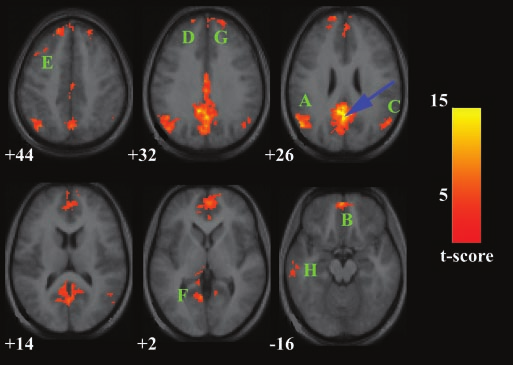
\includegraphics[height=5cm]{Pictures/fmri.png}
    \caption{Map of the resting-state neural connectivity for the PCC. The blue arrow indicates the approximate location of the PCC peak.}
    \label{fig5}
\end{figure}

\begin{figure}
    \centering
    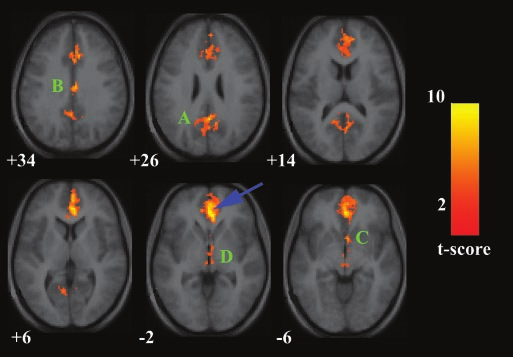
\includegraphics[height=5cm]{Pictures/fmri1.png}
    \caption{Map of the resting-state neural connectivity for the vACC. The blue arrow indicates the approximate location of the vACC maximum.}
    \label{fig6}
\end{figure}

\subsection{Research gaps}
    The DMN is routinely identified with functional magnetic resonance imaging (fMRI) or positron emission tomography (PET). However, both of these methods impose restrictions on the groups of patients that can be examined.Since, fMRI is not portable, and too expensive ,our work enables the characterization of DMN alterations in patient groups that are difficult to study with fMRI or PET

\subsection{Objective}
    The objective of my project is to show that the DMN can also be identified by electroencephalography (EEG). By instructing subjects to alternate between self-referential memory recall and focusing on their breathing induces a spatial pattern of spectral band power modulation in the $\theta$- and $\alpha$-band (4–16 Hz) that is consistent with the DMN pattern observed with PET and fMRI.
    In my study, i have developed a topological graph of head to show the activated brain regions during mind wandering state. 

\section{Default Mode Network in brain}
    Default mode network (DMN) is a large scale brain network of interacting brain regions known to have activity highly correlated with each other.DMN is most commonly active when a person is not focused on the outside world and the brain is at wakeful rest, such as during daydreaming and mind-wandering.Also active when the individual is thinking about others, thinking about themselves, remembering the past, and planning for future.The DMN has been shown to be negatively correlated with other networks in the brain such as attention networks.Fig 1.3 shows the parts for brain active during mind wandering state also called DMN.
    \begin{figure}
        \centering
        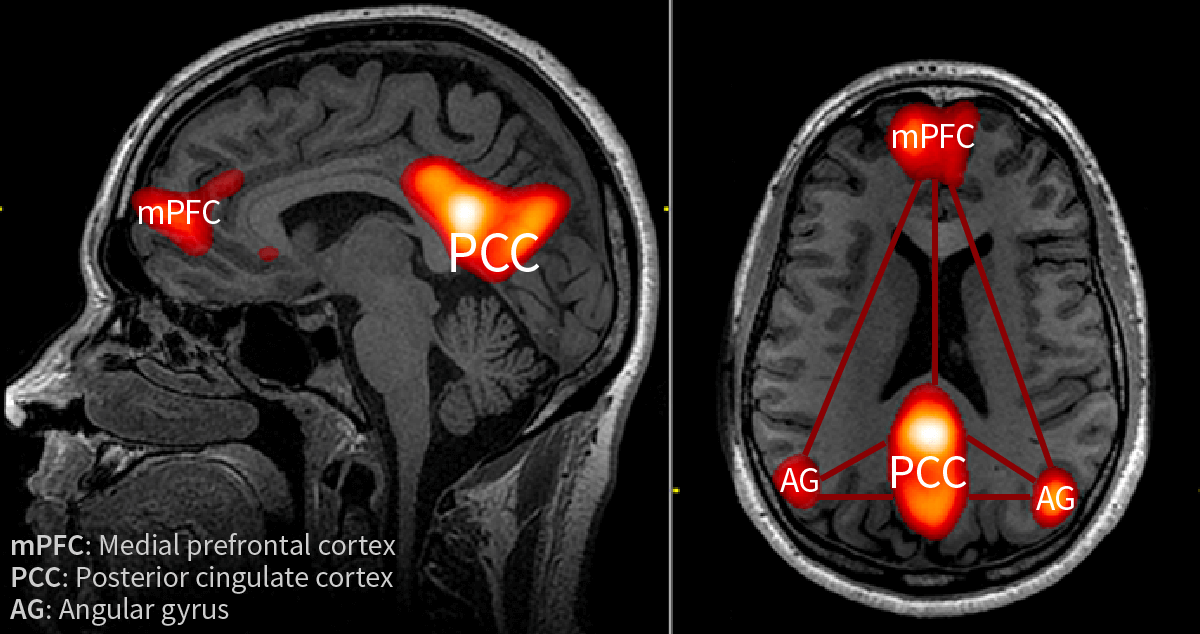
\includegraphics[height=7cm]{Pictures/dmn.png}
        \caption{fMRI scan showing default mode network [2]}
        \label{fig:my_label2}
    \end{figure}
\subsection{DMN anatomy}
Areas of the brain included in the default mode network include the medial temporal lobe, the medial prefrontal cortex, and the posterior cingulate cortex, as well as the ventral precuneus and parts of the parietal cortex. All of these regions have been associated with some aspect of internal thought. For example, the medial temporal lobe is associated with memory. The medial prefrontal cortex has been associated with theory of mind, the ability to recognize others as having thoughts and feelings similar to one’s own. The posterior cingulate is thought to involve integrating different kinds of internal thoughts. Mirror neurons have also been posited to interact with the DMN.
\begin{figure}
    \centering
    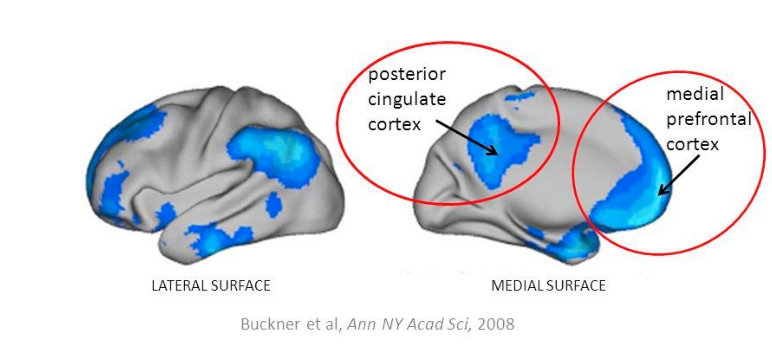
\includegraphics[height=6cm]{Pictures/DMN_anatomy.png}
    \caption{Brain regions included in DMN}
    \label{fig:my_label}
\end{figure}

The repeated observation that the ventral medial prefrontal cortex (vmPFC) and posterior cingulate cortex (PCC) paradoxically exhibit high levels of activity during resting baseline and decreases in activity during externally-oriented cognitive tasks led to the characterization of these regions as belonging to a “default mode network” (DMN) (Esposito, et al. 2006; Fransson 2006; Gusnard, et al. 2001a; McKiernan, et al. 2003; Raichle, et al. 2001). Originally proposed as a system for evaluating “information broadly arising in the external and internal milieu” (Raichle, et al. 2001), the network has since been posited to underlie a variety of functions. The DMN has been linked to episodic memory (Greicius and Menon 2004) and memory consolidation (Miall and Robertson 2006) in some studies, and social (Iacoboni, et al. 2004; Uddin, et al. 2005) or self-related processes (Buckner and Carroll 2007; Gusnard, et al. 2001a; Wicker, et al. 2003) in others. Still others associate default mode function with more general processes such as stimulus-independent (Mason, et al. 2007) or task-unrelated thought (McKiernan, et al. 2006). Though it is possible that one comprehensive theory will arise explaining the network’s ability to support such a diverse array of functions, the greater likelihood is that the default mode network consists of functionally differentiable subdivisions or subnetworks.

\paragraph{Posterior cingulate cortex (PCC) $\And$ precuneus: } The ventral (lower) part of PCC activates in all tasks related to the self, related to others, remembering the past, thinking about future, and processing concepts plus spatial navigation. The dorsal (upper) part of PCC involves involuntary awareness and arousal. [FIGURE 1.4]
% \begin{figure}
%     \centering
%     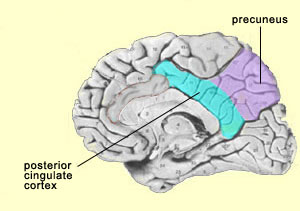
\includegraphics[height=7cm]{Pictures/pcc.jpg}
%     \caption{Posterior cingulate cortex (PCC) $\And$ precuneus }
%     \label{fig:my_label}
% \end{figure}

\paragraph{Medial prefrontal cortex (mPFC):} Decisions about self processing such as personal information, autobiographical memories, future goals and events, and decision making regarding those personally very close such as family. . [FIGURE 1.4]

\paragraph{Angular gyrus:} Connects perception, attention, spatial cognition, and action and helps with parts of recall of episodic memories.The angular gyrus is a region of the brain in the parietal lobe, that lies near the superior edge of the temporal lobe, and immediately posterior to the supramarginal gyrus; it is involved in a number of processes related to language, number processing and spatial cognition, memory retrieval, attention, and theory of mind. . [FIGURE 1.3]


\section{Data set}
The data set we are using has been collected during an another study [3].So, i am describing the method of data collection here of that data.
\paragraph{Subjects :}
   Two participants S1 female (age 25) and S2 male (age 31) volunteered for this experiment after providing written informed consent.Both participants had normal or corrected to normal vision. They were both right handed and reported no mental or neurological disorder. The two subjects did not receive any monetary compensation for their participation. The experimental protocol was approved by the local ethical committee (CPP 2010-A00744-35). Both subjects had performed the task before and had been practicing meditation.To accumulate enough mind wandering data, each subject performed 10 sessions of 20 min each over the course of about 5 weeks.
\paragraph{Procedure:}
    Subjects sat in a dimly lit room with their heads on a chin rest. Instructions were displayed at the beginning of each session on the screen placed at 60 cm in front of them.The task of the subjects was to count backward each of their breath cycles (inhale/exhale) from 10 to 1. At 1, they were instructed to restart counting backward from 10.Subjects also had to indicate whenever they realized they had lost track of their breath count (i.e., that their attention had drifted) by pressing the left mouse button.Immediately following the button press, a short 1-page phenomenological questionnaire was presented on the computer screen. The questionnaire allowed the subject to characterize their mind wandering episodes. After the questionnaire was completed, subjects had to press the right mouse button to indicate they were ready to restart the breath counting task.EEG data were recorded using a 64-channel Bio-semi Active Two system.
    
\section{Data processing}
 Data is collected using EEG.It also contains alert state data along with mind wandering state data.So, we have to select only mind-wandering state data.And to see the desired result we have to follow some steps that are shown in Figure 1.5.  
 \begin{figure}
    \centering
    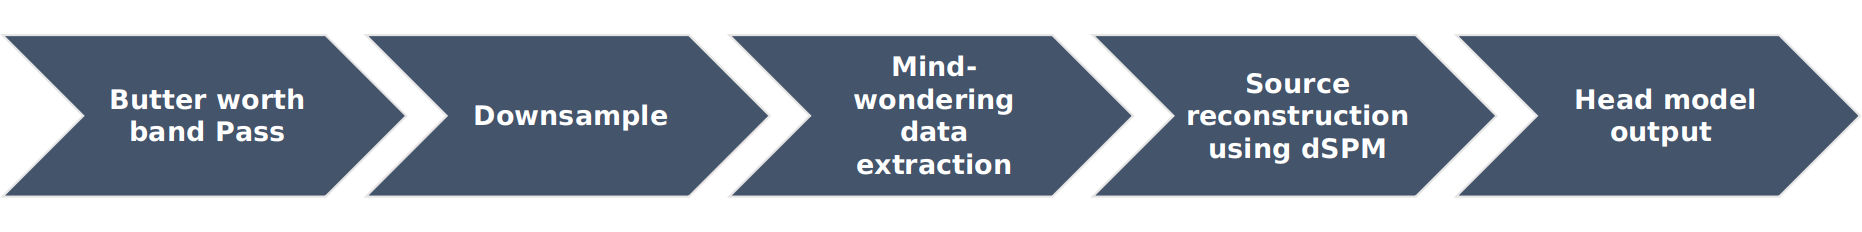
\includegraphics[width=15cm]{Pictures/Picture2.png}
    \caption{Steps of data processing}
    \label{fig:my_label1}
\end{figure}
\subsection{Prepocessing}
    \paragraph{Band Pass Butter worth filtering:} By comparing source  activation levels, we found $\theta$- and $\alpha$ band power changes in the medial prefrontal cortex, the posterior cingulate cortex, and the temporoparietal junction - a pattern that is highly consistent with the DMN. So,for our study we are focusing on the $\theta$ -band (3.5Hz-7Hz) and $\alpha$ -band (8-14 Hz).We restricted our analysis to a combination of $\theta$ and $\alpha$ frequency bands (4–16 Hz, individually adjusted for each subject). The lower $\theta$ boundary was set to 4 Hz for all the subjects, while the upper $\alpha$ boundary was set to 14Hz.
    \paragraph{Down sampling :}
    The data was then band-pass filtered with a 3rd order Butter-worth filter in the $\theta$-and in the $\alpha$- frequency band, respectively.The sampling rate of original data was 1024Hz.With this sampling rate it was not quite possible to process data further.SO,we have down-sampled data to 256 Hz.We decided down-sampling rate  by keeping information loss factor in mind. 
    \paragraph{Mind wandering data extraction:}
    The data was collected continuously.SO, it was contaminated with alertness data.During the data collection subjects had to press button when they realized that they were lost.So, we considered that it took 2 seconds of time to realize and press the button.And we also considered that subject was in mind-wandering state at least for 4 seconds.For mind-wandering data, we extracted data from -6 to -2 seconds where button press event occured at 0 second.

\subsection{Source reconstruction using dSPM}
    To project the sensor activation on the source level, we applied Dynamic Statistical Parametric Mapping,a noise-normalized minimum norm estimate, to the preprocessed data.We generated the forward model with the BrainStorm toolbox,using standardized electrode locations and a standardized three-shell spherical head model. Then, the activity of each source was estimated from the measurements of the electrical potential on the surface of the scalp at all electrodes.We then estimated a noise-normalized current dipole power at each time point and location . We made no assumptions on dipole orientation and thus averaged three dipoles for each location:

\section{Results}

\begin{figure}
    \centering
    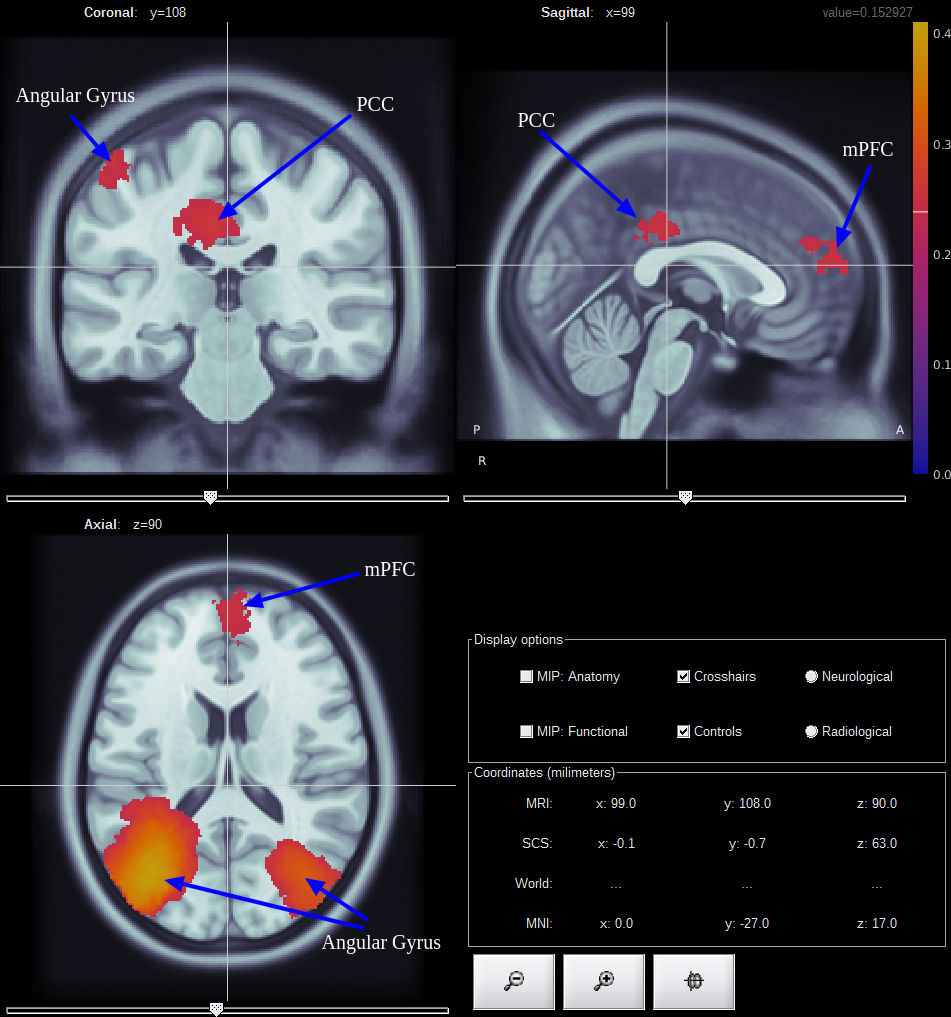
\includegraphics[width=15cm]{Pictures/result1.png}
    \caption{The Default Mode Network (DMN) identified with EEG.Orange shows positive correlation with
the autobiographical memories condition}
    \label{fig:my_label3}
\end{figure}
Figure 1.6 displays the sources that we found to show a statistically significant modulation on the group-level. We find the most prominent modulation of band power in the posterior cingulate cortex (PCC),which constitutes a hub of the DMN . In addition, we observe band power modulation in the medial prefrontal cortex (mPFC) and in the left temporoparietal junction. With the exception of the right temporoparietal junction, our method thus identifies the core areas of the DMN.

\section{Discussion}
We identified a pattern of EEG band power modulation consistent with the characterization of  DMN with PET and fMRI using the cognitive strategy of alternating autobiographical memories and focusing on breathing. For two reasons, this is particularly important. First, this EEG-based identification of DMNs enables us to study the oscillatory properties of DMNs that are not accessible by PET or fMRI. And second, our work makes it possible to study DMN changes in the patient.

Nevertheless, we note that, despite the fact that fMRI has a higher spatial resolution, the EEG-based DMN nodes are smaller than those identified by fMRI. The low spatial resolution of EEG source localization methods is one potential reason for this observation. The spatial variation between individual DMN patterns may be smaller than each individual DMN pattern on its own due to differences in head shape and cortical folding between subjects. This can contribute to a spatial underestimation of the DMN at group level. Using individualized EEG forward models derived from structural MRI scans may address this problem.
% \begin{figure}
% \centering
% 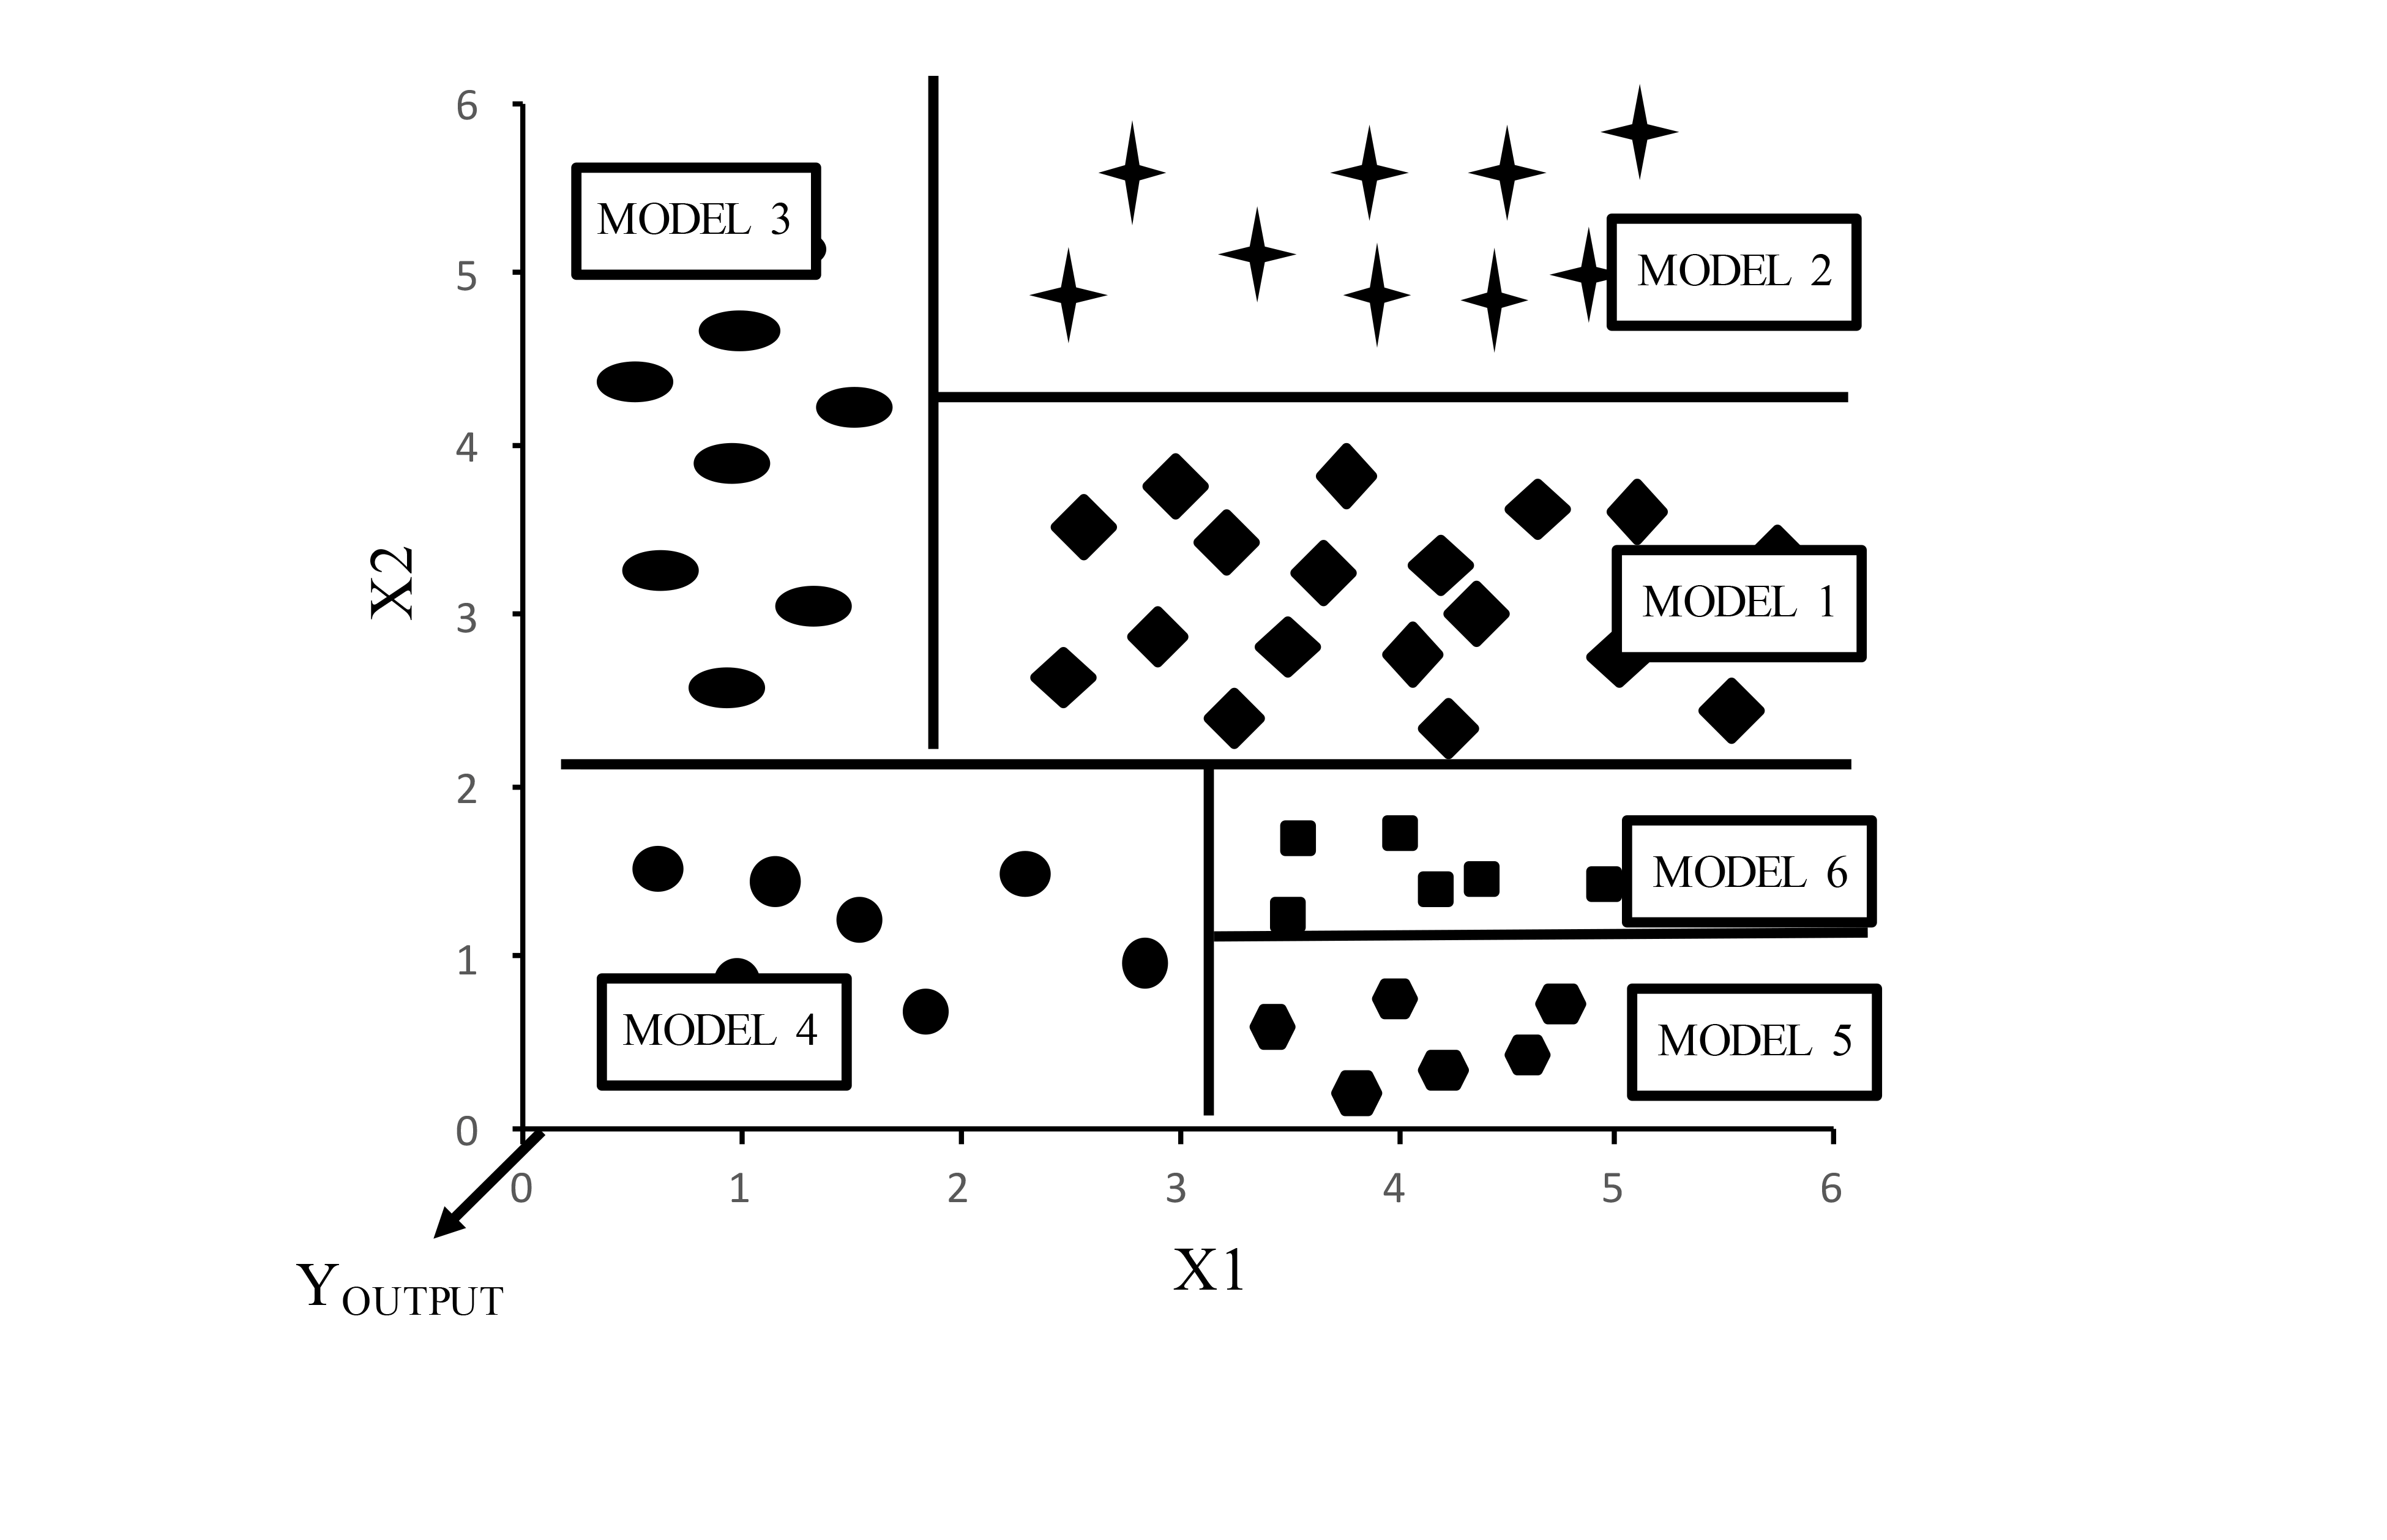
\includegraphics[height=7cm]{splits.png}
% \caption{Splitting of the input space (X1 x X2) by M5' model tree algorithm}
% \label{fig7}
% \end{figure}

% \section{Adding another section}
% You can show a lot of figures together like these Figures \ref{fig61}, \ref{fig62}, \ref{fig63} below.
% \begin{figure} [!htbp]
% \centering    
% \subfigure[Caption1]{\label{fig61}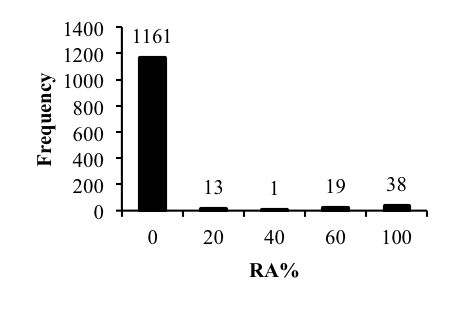
\includegraphics[width=42mm]{data1.png}}
% \subfigure[Caption2]{\label{fig62}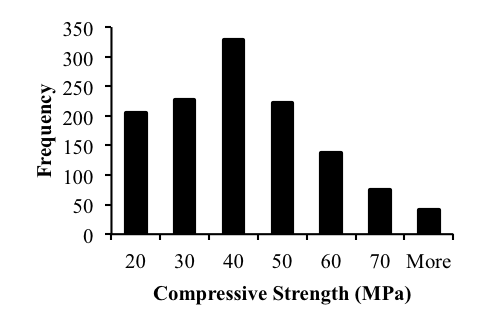
\includegraphics[width=42mm]{data2.png}}
% \subfigure[Caption3]{\label{fig63}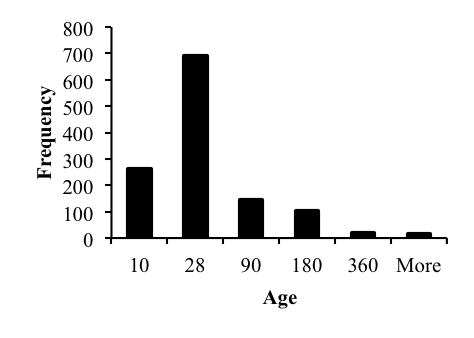
\includegraphics[width=42mm]{data3.png}}
% \caption{Figures sample}
% \end{figure}
% You can add lists into the text like this. 
% \begin{itemize}
% \settowidth{\leftmargin}{{\Large$\square$}}\advance\leftmargin\labelsep
% \itemsep3pt\relax
% \renewcommand\labelitemi{{\lower1pt\hbox{\small$\square$}}}
% \item	Some sample text item 1. 
% \item You may refer to tables \ref{tab1} 
% \item Or figures \ref{fig61}
% \end{itemize}

% Tables can be added like this
% \begin{table}[!htbp]
% \centering
% \caption{Sample table}
% \label{tab1}
% \begin{tabular}{llll}

% \hline
% Column 1 & Column 2 & Column 3       \\\hline
% 1         & Data1 & 13.41179 & 0.9492839 \\
% 2            & Data2 & 13.39824 & 0.9492952\\\hline
% \end{tabular}
% \end{table}



% Chapter Template

\chapter{Introduction} % Main chapter title

\label{Chapter1} % Change X to a consecutive number; for referencing this chapter elsewhere, use \ref{ChapterX}

\lhead{Chapter X. \emph{Introduction}} % Change X to a consecutive number; this is for the header on each page - perhaps a shortened title

%----------------------------------------------------------------------------------------
%	SECTION 1
%----------------------------------------------------------------------------------------
\section{Electroencephalogram}
An electroencephalogram (EEG) used in evaluation of the brain neuron's electrical activity  . Brain cells uses electrical impulses to communicate to each othe.

An EEG measures electric field fluctuation induced by the  number of electron fluctuation during the neuron communication.The change in the voltage at any reason of brain shows the activity of that region of brain.The measured voltage has to amplified as the is too small in value.The electrodes has been used to measure the voltage,also called channels.In the Figure \ref{fig:eeg},you can see the electrodes are mounted on human brain.
 \begin{figure}
     \centering
     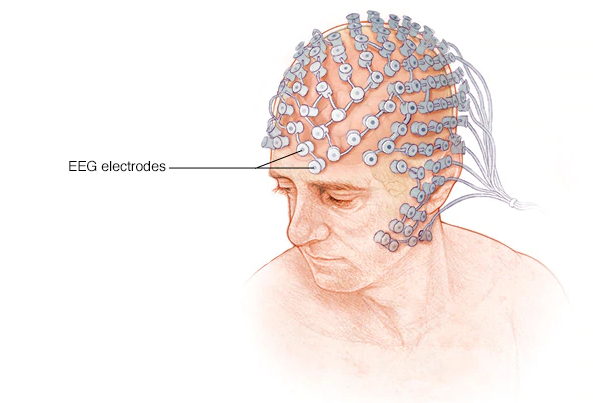
\includegraphics[width=15cm]{Pictures/eeg_1.png}
     \caption{An Image of EEG, showing electrodes \cite{eeg} }
     \label{fig:eeg}
 \end{figure}
\section{Mind Wandering (MW)}
Mind Wandering (MW) is the self-generated thoughts drifting our mind away from the current task. It is a psychological phenomenon that is diverting our attention from a task. MW usually happens while driving \cite{baldwin2017detecting}, reading and other activities where there is less attention. It is a temporary state and is a common trait that people share where they do not remember what was going on in their surroundings since their minds were decoupled. MW can both be intentional and unintentional \cite{seli2017intentionality}. While MW is a common phenomenon, it relates to various psychological problems too.

MW covers about 30-50\% of the waking time which is known to be initiated from the transitions between outwardly steered and self-generated thoughts .EEG is a well-accepted tool in detection of MW to identify artifacts from multi-channel EEG data . It has a few limitations in measuring circumstance, and a passable amount of information is expected. In un-investigated conditions the EEG indicator can divulge the nature of MW.As MW tends to occupy half of our waking time it plays a crucial role in our everyday life. Indeed there are benefits to MW . MW is an essential measure of our self-identity and has also been knotted to creative problem-solving . It results in helping us make plans about the future. MW enhanced human’s creativity above and beyond the positive effects of their reading ability or fluid intelligence, the general ability to solve problems or puzzles . Admittedly, it was found that happiness of a person who is in MW decreases suggesting that a negative mood might be a consequence  of a wandering mind. Besides, it is a menace to transportation safety, resulting in substantial number of crashes and fatalities . Taken together whether MW is good or bad depends on when we mind wander and what we wander about .

Furthermore, reviewing the prior research under this field, a good sum of work has been dedicated in detection of MW. There are numerous existing research works employed to extract various features such as EEG variables and non-linear regression , oculometric features \cite{grandchamp2014oculometric}, incubation paradigm to assess performance , oscillatory activity of the entire brain , spontaneously adopted problem solving approaches using self-reports , kernel size and stride , EEG markers used as features for the classifier  spatial patterns to discover scalp topologies 

\section{Aims And Objectives}

In this project, we explored basic machine learning techniques to predict the mind wandering using EEG signals.In order to achieve a higher accuracy, classification of different combinations of features were done.XgBoost gave a higher accuracy than random forest so applying two classification methods aided our precision level. The main factor in our paper is that we have worked with EEG signals solely to detect MW and has also achieved a promising result which thus elevated our method over other research method under this field.

% Chapter Template

\chapter{Literature Survey} % Main chapter title

\label{Chapter2} % Change X to a consecutive number; for referencing this chapter elsewhere, use \ref{ChapterX}

\lhead{Chapter 3. \emph{Literature Survey}} % Change X to a consecutive number; this is for the header on each page - perhaps a shortened title
Human mind is not static; it fluctuates over time especially in an attention demanding task. When our brain fluctuates, our mind works in both task-relevant and irrelevant processes but in a less detailed manner.\cite{grandchamp2014oculometric}, We have worked on detecting wandering of our mind using EEG signal in which electrical activity of the brain has been recorded using an electro physiological method. We have also observed the brain waves in EEG signal in the frequency domain. Among various classifiers we have used J48 algorithm to generate a decision tree from our featured data. For classification we have used SVM classifier. By giving a set of trained data example SVM built a model that assigned our data’s in positive or negative MW categories. 

Few researchers also have worked on this field. Julia W. Y. Kam Julia et al. \cite{kam2013mind} have used two experiments, in one experiment they have used traditional measures of performance  and found that both automatic and volitional and  forms of visual–spatial consideration arranging were fundamentally constricted when MW episodes occurred. In the second experiment ERPs have used to examine whether time frames wherein we momentarily weaken the preparing of outer improvement contributions as our considerations float away from the on-going main job or cortical hypersensitivities in headaches reach out to MW.Another group Romain Grandchamp et al. \cite{grandchamp2014oculometric} worked on oculometric variations during MW. They have worked on blink frequency, pupil size and gaze position to check if they were correlated with the occurrence and time course of self-reported MW episodes. 

Another group Jaechoon et al have worked on online education limitations by performing a verification study to see if  mind wandering can be detected using high frequency words to resolve limitations that currently exists. They established a Minimum Learning Judgment System (MLJS) in which vido-based online lecture has been used to detect Mind wandering. 

One more group Benjamin W. Mooney- hamet al.have worked on Mind states by analysising the Neural Bases of alertness and Mind wandering through a dynamic FC. They have used Electrophysiological recordings, EEG data processing, event-related potential and phase locking factor[26-27]. Yuyu Zhang et al.[28] in their research Automatic detection of MW in a simulated driving task with behavioral measures have measured accuracy of 72\% by driving behavior measurements to automatically detect MW state in the driving task. Another group Benjamin Baird et al. [29] and others have worked on decoupled mind by processing EEG data and have found MW disrupts cortical phase-locking to perceptual events. Todd C. Handy[30] and others have worked on MW and selective attention to the external world. The main focus of their work is visual attention, executive function and mental simulation [31-34]. Another group Jonathan Smallwood et al [35] has examined whether the periods of mind wandering are associated with reduced cortical analysis of the external environment. 

Julia W.Y. Kam et al.[34] researched about how the Brain allows us to mentally wander off to another time and place. Kiret Dhindsa et al. [9] have worked on Individualized pattern recognition for detecting MW from EEG during live lectures. They have recorded EEG simultaneously from 15 participants during live lectures and used a data-driven method known as common spatial patterns to discover scalp topologies for each individual that reflects their differences in brain activity when MW versus attending to lectures and achieved an average accuracy of 80-83\%. Jin CY et. Al. [43] have worked on Predicting task-general MW with EEG. They have classified the participants current state by two different paradigm, one is sustained attention to response task (SART) and a visual search task to detect either MW or on task. Qin et al. [44] haveworked on Dissociation of subjectively reported and behaviorally indexed MW by EEG rhythmic activity. By implementing time frequency analysis and means of beamformer source imaging they have found that found subjectively reported MW within the gamma band to be characterized by increased activation in bilateral frontal cortices, supplemental motor area, paracentral cortex and right inferior temporal cortex in comparison to behaviorally indexed MW. Compton RJ ET AL. [45] have worked on the wandering mind oscillates: EEG alpha power is enhanced during moments of MW. During a demanding cognitive task, to find whether episodes of MW increases in EEG alpha power they have used a within-subjects experience-sampling design. 

In the research of Kiret et al.[9] the drawbacks of their work was with only 16 EEG signals they lack the spatial pattern needed for accurate source localization. MW has been mainly detected through two thought-report methods: discrete thought-
probes [49-51] and spontaneous self- reports [49].

A method that have been used is spontaneous self-reports. In this method par- ticipants are requested to specify the moment when they become conscious of MW. From the participant’s side, this method continuously track of MW. This method limits the ability of researchers to maintain consistent evaluation among different participants. We have overcome this problems through our work and analysis.

% Chapter Template

\chapter{Data set} % Main chapter title

\label{Chapter3} % Change X to a consecutive number; for referencing this chapter elsewhere, use \ref{ChapterX}

\lhead{Chapter 3. \emph{Data set}} % Change X to a consecutive number; this is for the header on each page - perhaps a shortened title
The data set we are using has been collected during an another study [3].So, i am describing the method of data collection here of that data.The dataset utilized in this project was tailored from a French research groups work on oculometric changes in MW episodes, Braboszcz and Delorme \cite{grandchamp2014oculometric} and was open to all for EEG analysis under “CeCILL v2.0” license.
%----------------------------------------------------------------------------------------
%	SECTION 1
%----------------------------------------------------------------------------------------

\section{Subjects}
There was two  volunteer participants after providing written informed consent for this experiment.There was two volunteers,one of them was a 25 years old female (say S1)  and another was  a 31 years old male  (say S2) \cite{grandchamp2014oculometric}.Both of them had a normal vision. Both them had  no neurological or mental disorder and both of them are right handed. For their participation,there was no monetary compensation has been provided .The local ethical committee (CPP 2010-A00744-35) had approved  the protocol followed in procedure of data acquisition  \citet{grandchamp2014oculometric}. Both subjects had been practicing meditation and had performed the task before .To accumulate enough data,each subject had to perform 10 sessions, each session was about 20 minutes.The data was collect over course of 5 weeks \cite{grandchamp2014oculometric}.
%-----------------------------------
%	SUBSECTION 1
%-----------------------------------
\section{Procedure}
 
 \begin{figure}
    \centering
    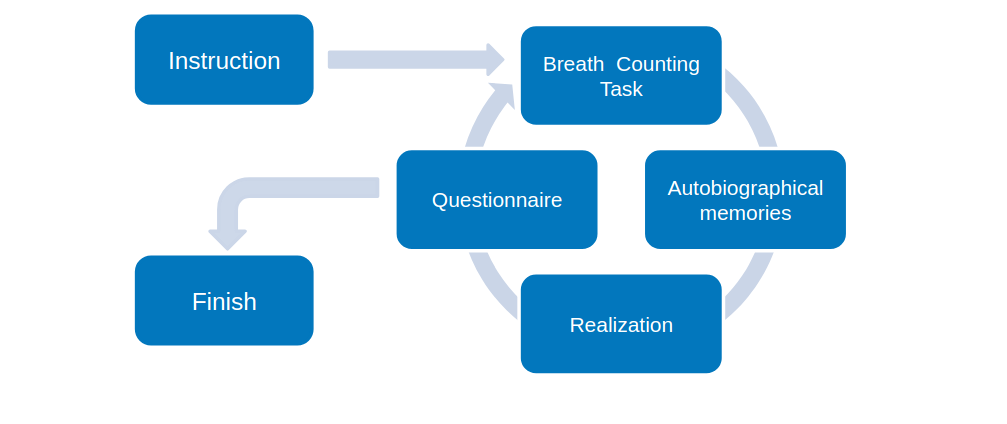
\includegraphics[width=15cm]{Pictures/data_collection.png}
    \caption{data collection flow diagram }
    \label{fig:data_collection}
\end{figure}

The subjects (1 male , 1 female) performed their given task in a dimly lit and soundproof space ahead of a visual display unit .On the display, there were instructions at the beginning of each session.A breath counting task have be performed by the two subjects .They had to count their breath in backward cycles (one inhale and one exhale) from 10 to 1 as one of them reported forward counting even when they were unconscious.By pressing the button,they had to report whenever they realized that they had lost track of their breath count.After button press, a questionnaire were presented on the screen immediately. It took less than 60 seconds to complete the questionnaire and after the participant's indication process resumed again.A total of 20 session were recorded each of about 20 minute. Using a BioSemi EEG system, EEG signals are recorded from 64 scalp channels from BCI device (an elastic cap) and different biometric channels are concerned in remainder of the channel information recordings. Initial sampling rate of data recording was 1024Hz. Skin Conductance (SC), Electrocardiogram (ECG), further as eye movements and pupil size were additionally recorded. By performing these procedures 19 sessions were recorded of 2 subjects. In this 80 channeled dataset first 64 channels are EEG channels and remainder of the channels are other biometric channels like Pupil size , Gaze position , Skin conductance (SC),Electrocardiogram (ECG) etc. In our paper we only present the findings on EEG information basis .
%  Subjects sat in a dimly lit room with their heads on a chin rest. Instructions were displayed at the beginning of each session on the screen placed at 60 cm in front of them.The task of the subjects was to count backward each of their breath cycles (inhale/exhale) from 10 to 1 \cite{grandchamp2014oculometric}. At 1, they were instructed to restart counting backward from 10.Subjects also had to indicate whenever they realized they had lost track of their breath count (i.e., that their attention had drifted) by pressing the left mouse button.Immediately following the button press, a short 1-page phenomenological questionnaire was presented on the computer screen \cite{grandchamp2014oculometric}. The questionnaire allowed the subject to characterize their mind wandering episodes. After the questionnaire was completed, subjects had to press the right mouse button to indicate they were ready to restart the breath counting task.EEG data were recorded using a 64-channel Bio-semi Active Two system \cite{grandchamp2014oculometric}. Figure ~\ref{fig:data_collection} and Figure ~\ref{fig:single_chanel_data} shows the flow chart of the data collection process.And you can see a sample of collected data in Figure ~\ref{fig:data_sample},blue line indicated by an arrow shows a button click event.


 
 \begin{figure}
    \centering
    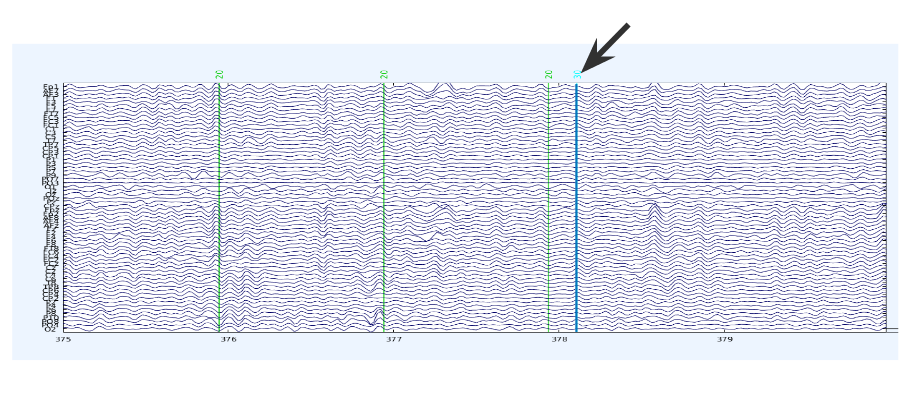
\includegraphics[width=15cm]{Pictures/data_sample.png}
    \caption{A sample of collected data (64 channels) }
    \label{fig:data_sample}
\end{figure}

 \begin{figure}
    \centering
    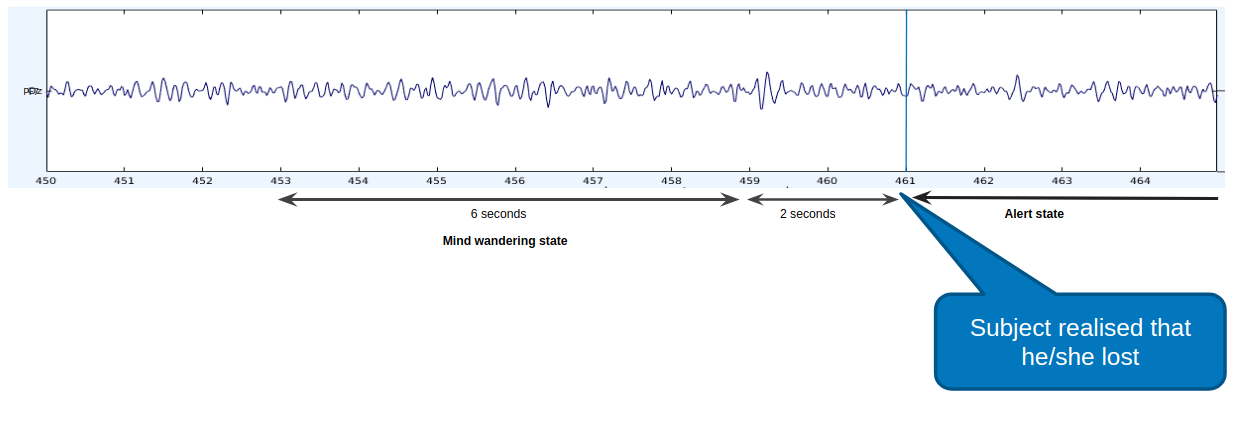
\includegraphics[width=15cm]{Pictures/single_chanel_data.png}
    \caption{Data of a single channel }
    \label{fig:single_chanel_data}
\end{figure}
 
% Chapter Template

\chapter{Work Procedure} % Main chapter title

\label{Chapter4} % Change X to a consecutive number; for referencing this chapter elsewhere, use \ref{ChapterX}

\lhead{Chapter 4. \emph{Work Procedure}} % Change X to a consecutive number; this is for the header on each page - perhaps a shortened title

%----------------------------------------------------------------------------------------
%	SECTION 1
%----------------------------------------------------------------------------------------
The aim of the this project is to detect the MW phase of mind more precisely with lowest false alarm. A set of steps have been followed to complete the procedure. A diagram has been given to illustrate in Figure ~\ref{fig:work_procedure} with a comprehensive description given in section. Data pre-processing,Normalization feature extraction, and classification are the basic steps to train a model and classify the MW phase.


\begin{figure}
    \centering
    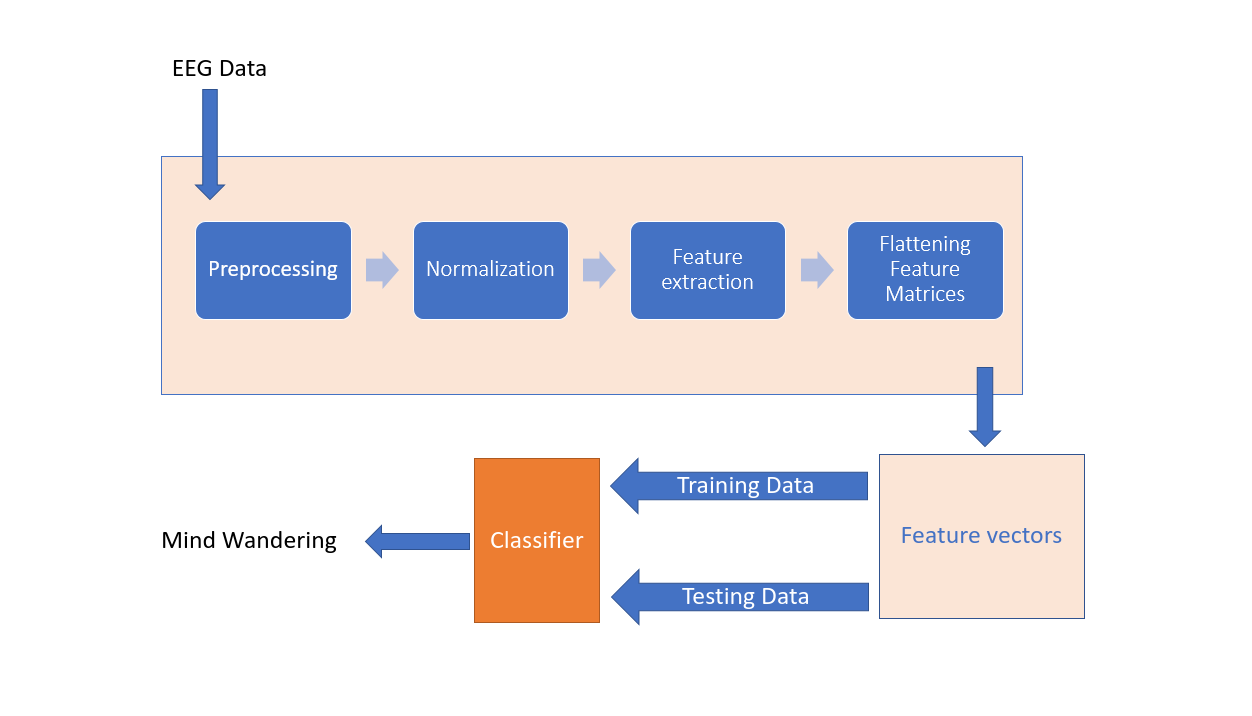
\includegraphics[width=15cm]{Pictures/workprocedure.png}
    \caption{Work Procedure }
    \label{fig:work_procedure}
\end{figure}

\section{Data Pre-processing}

Data was recorded from 64 channels with 1024 Hz sampling rate.By comparing source  activation levels,a significant change in the power of the  $\theta$- and $\alpha$ band observed in the MPC, the PCC, and the temporo-parietal junction (In MTP-I). So,we focused on the $\theta$ band (3.5Hz-7Hz) and $\alpha$ -band (8-16 Hz) in our study.We limit our study to  $\alpha$ and $\theta$  frequency bands that is 3–16 Hz. The lower $\theta$ band frequency boundary was set to 3 Hz for both subjects, while the upper $\alpha$ band frequency boundary was set to 16 Hz. Then all the questionnaire sessions were removed from the data. Channel signals containing  electrical and eye blink artifacts (as assessed by visual inspection) or high frequency noise were removed and clean data set reformed. Then the signal was converted to average reference level .Lastly , data set was normalized for data mining.
 
\begin{figure}
    \centering
    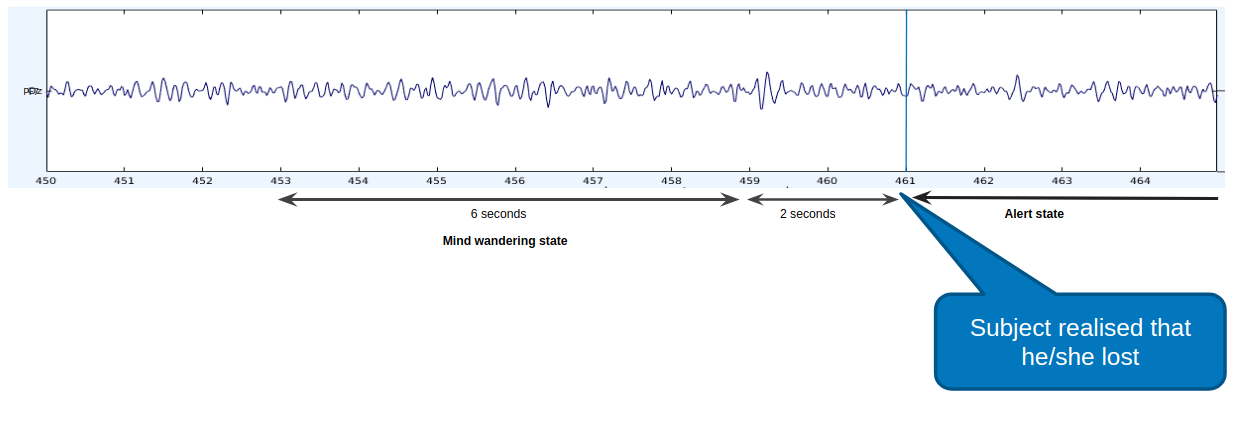
\includegraphics[width=15cm]{Pictures/single_chanel_data.png}
    \caption{Button press event,Alertness and Mind wandering}
    \label{fig:Mw_fig}
\end{figure}

\subsection{Alertness and MW data extraction}
 The data was collected continuously.So, it was contaminated with alertness data.During the data collection subjects had to press button when they realized that they were lost.So, we considered that it took 2 seconds of time to realize and press the button.And we also considered that subject was in mind-wandering state at least for 4 seconds.For mind-wandering data, we extracted data from -6 to -2 seconds as MW state and 2 to 6 seconds as alertness state where button press event occured at 0 second.All the events and time laps illustrated in Figure ~\ref{fig:Mw_fig}.
 
As a result of above procedure, we got 977 files containing a 2D matrix each correspond to either MW or Alertness.A row contains data of a channel collected in 4 seconds that is 4X1024 samples.There were 64 channels and each channel has 4096 readings.Each 2D matrix has dimension of 64 X 4096.   

\section{Normalization}
The Z-score normalization method has been used to normalize the EEG samples collected during breath counting task. Samples were normalized to have a standard deviation of 1 and a zero mean . The dimension of our dataset is [977,64,8192](total sample,\# channels,total time instances). It means there are 977 samples of dimension [64,8192] each. So mean and standard deviation were calculated for all signals. We normalized the  training samples by subtracting the mean and dividing the result by standard deviation.The standard deviation and Mean of training set have been stored in a file to later normalize the testing and validation set.

\section{Feature extraction}
To reduce the dimension we used feature extraction method.In the process of feature extraction,the relevant information to perform a desired task is expected to keep,instead of keeping complete information.Our data-set consist of 19 sessions containing specific task related to our investigation. This sessions was acquired from two subjects. Then we used built in methods of MATLAB and various Python libraries to extract features, which are mentioned below:


\begin{itemize}
    \item Coefficient of variation
    \item first difference
    \item slope mean
    \item slope variance
    \item kurtosis
    \item second difference mean
    \item second difference max
    \item skewness
    \item first difference mean
    \item first difference max
    \item fractal dimension
    \item Auto regressive model parameters 
    \item Hjorth parameters
    \item wavelet features
    
\end{itemize}
\subsection{Coefficient of variation}
The statistical measure of the dispersion of date instances  around the mean a data set is called coefficient of variation (COV) . The coefficient of variation represented by the ratio of standard deviation to the mean. And the usefulness of COV statistic is to compare the degree of variation two data series , even if they have drastically different means .
\begin{equation}
 \label{coeff_var}
 \begin{split}
    C_v = \frac{\sigma}{\mu}  
 \end{split}
\end{equation}

Where :
$$\sigma = Standard Deviation  $$
$$\mu = mean$$

\subsection{First Difference}
First difference is an array containing difference of previous element with the current element.
\begin{lstlisting}[language=Python]
def first_diff(i):
    b=i
    out = np.zeros(len(b))
    for j in range(len(i)):
        out[j] = b[j-1]-b[j]# Obtaining the 1st Diffs
        j=j+1
        c=out[1:len(out)]
    return c #returns first diff
\end{lstlisting}

\subsection{slope mean}
First we calculated slopes of each row using maximum and minimum amplitude, then we took mean of all slopes. 
\subsection{slope variance}
We calculated slope using above method then we calculated variance of slopes.  
\subsection{Skewness}
The measure of the distortion degree from  the normal distribution or the symmetrical bell curve, is the Skewness. It measures the feeble amount of balance of parts, same on 2 sides in data distribution.Zero Skewness indicates a symmetrical distribution.\\
Figure \ref{fig:skewness} shows the Skewness result of our subject 1 task 1 in .
\\
Types of Skewness: Negative and Positive\\
 The  right side tail of the distribution is quite longer or fatter than the left side tail in positive skewness. The mode will have lesser value than mean and median.\\
 The  right side tail of the distribution is quite smaller or thinner than the left side tail in negative skewness. The mode will have greater value than mean and median.
\begin{figure}
    \centering
    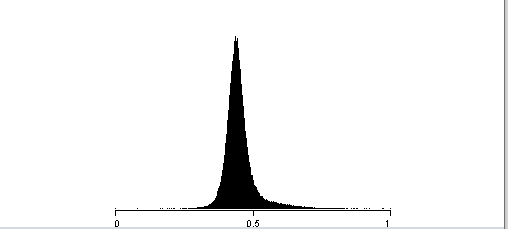
\includegraphics[width=15cm]{Pictures/skewness.png}
    \caption{Skewness result}
    \label{fig:skewness}
\end{figure}
\subsection{Kurtosis}
Kurtosis is the measure of the tails of the distribution,it is not about the  flatness or the peakedness.  To outline the uttermost values in one vs the other tail,kurtosis has been used.Basically  Kurtosis is the measure of outliers  of the distribution.We have shown the sample Kurtosis graph,in the Figure \ref{fig:kurtosis} .
\begin{figure}
    \centering
    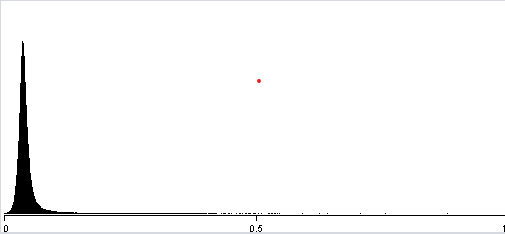
\includegraphics[width=15cm]{Pictures/kurtosis.png}
    \caption{Kurtosis:sample diagram}
    \label{fig:kurtosis}
\end{figure}
\subsection{First difference mean}
First difference mean is the average of  first difference of an array.where,First difference is an array containing difference of previous element with the current element.
\begin{lstlisting}[language=Python]
def first_diff_mean(arr):
    data = arr 
    diff_mean_array = np.zeros(len(data)) #Initialinling the array as all 0s
    index = 0; #current cell position in the output array
    for i in data:
        sum=0.0#initializing the sum at the start of each iteration
        for j in range(len(i)-1):
            sum += abs(i[j+1]-i[j]) # Obtaining the 1st Diffs
        diff_mean_array[index]=sum/(len(i)-1)
        index+=1 #updating the cell position
    return np.sum(diff_mean_array)/1
\end{lstlisting}

\subsection{First difference max}
First difference max is the maximum value in first difference array.where,First difference is an array containing difference of previous element with the current element.
\begin{lstlisting}[language=Python]
def first_diff_max(arr):
    data = arr 
    diff_max_array = np.zeros(len(data)) #Initialinling the array as all 0s
    first_diff = np.zeros(len(data[0])-1)#Initialinling the array as all 0s 
    index = 0; #current cell position in the output array
    for i in data:
        max=0.0#initializing at the start of each iteration
        for j in range(len(i)-1):
            first_diff[j] = abs(i[j+1]-i[j]) # Obtaining the 1st Diffs
            if first_diff[j]>max: 
                max=first_diff[j] # finding the maximum of the first differences
        diff_max_array[index]=max
        index+=1 #updating the cell position
    return np.sum(diff_max_array)/1
\end{lstlisting}

\subsection{Fractal dimension (FD)}
The entropy measures the randomness of a dataset.The information in a data depends on entropy. Fractal dimension is related with the entropy \cite{Boostani_2004}.Thus, from fractal dimension we can interpret the degree of  signal irregularity or signal roughness . There are two famous methods to calculate fractal dimension,that are Peterson, Katz and Higuchi methods. the Katz method has  more  robustness[11] than others, and that is why we have used this in our project. Katz methods can derives from waveform directly. The  fractal dimension curve is defined as:
$$
FD = \frac{\log_{10} L}{\log_{10} d}
$$

here,\\
$L$ : curve length \\
and \\
$d$ : diameter \\
The diameter of curve is the distance between the farthest point of the curve and the  first point of sequence. \cite{Boostani_2004}.


\subsection{Auto regressive model parameters}
We have used the whitening lattice-filter method of Burg  to calculate the coefficients of an auto-regressive (AR) model of complex data (say x) \cite{burg1968new}. The inverse of the model is a moving-average filter which reduces x to white noise. The power spectrum of the AR model is an estimate of the maximum entropy power spectrum of the data \cite{burg1968new}.

\subsection{Hjorth parameters}

These parameters elaborates the  characteristics of signal. The measure of mean frequency, deviation from sin shape and variance of signal are used to describe the  characteristics of the signal.These terms are usually called activity, mobility and complexity respectively and  are  described as follows :
$$
Activity(x)=\frac{\sum^N_{i=1} (x(i) - \mu)^2}{N}
$$
$$
Mobility = \sqrt{\frac{VAR(x')}{VAR(x)}}
$$
$$
Complexity = \frac{Mobility(x')}{Mobility(x)}
$$

where,\\
$x$ : signal, \\
$x'$: signal derivative , \\
$N $:  \# samples  \\
$\mu$ : mean of signal\\
The  window  of calculation,we have used  for these parameters is  of size 500 ms without any overlapping.


\subsection{Wavelet features}
We have calculated mean,standard deviation,energy,entropy etc. with approximation coefficients and details coefficients for each channel. The minimum, maximum and mean of all these factors make a total of 24 features which contribute in the classification of MW.
\section{Flattening Feature Matrices}
We got 52 features for each channel signal.At the end we got 2D matrices with 64 $\times$ 52  (each row contains features of a  channel).The general form of a feature vector shown below:
\begin{align*}
&\boldsymbol{ch_1:} &f_1^1&,&f_1^2&,&f_1^3 &......    &f_1^{52} \\
&\boldsymbol{ch_2:} &f_2^1&,&f_2^2&,&f_2^3 &......   &f_2^{52} \\
&  \boldsymbol{.}       &.   &,  &. &, &.    &......   &.      \\
&  \boldsymbol{.}       &.   &,  &. &, &.    &......   &.      \\
&  \boldsymbol{.}       &.   &,  &. &, &.    &......   &.   \\
&\boldsymbol{ch_{64}:} &f_{64}^1&,&f_{64}^2&,&f_{64}^3 &......&f_{64}^{52} \\
\end{align*}

$\boldsymbol{ch_i :}$ feature  vector generated from the $i^{th}$ channel signal \\
$\boldsymbol{f_q^p :}$ $p^{th}$ feature of $q^{th}$ channel signal

Instead of using the 2-dimensional features vector to train machine learning models we have flattened them in to 1D vector.To flatten them we concatenated the each row into it's previous row except the first one.Thus,feature vector got flattened without loosing any information.we saved the reference of locality. 
The resulting in feature vector shown below:
\begin{align*}
    &\boldsymbol{Flattened \; feature \; vector:} &ch_1&,&ch_2&,&ch_3 &...... &ch_{64}
\end{align*}
$$or$$
\begin{align*}
&\boldsymbol{Flattened \; feature \; vector:} &f_1^1&,&f_1^2&,&f_1^3 &......    &f_1^{52}......&f_{64}^{52} \\
\end{align*}
The meaning of all symbols are same as defined above.

At the end of each row we have concatenated the label of each matrix as it was (1 for MW and 0 for Alertness state)
\section{Models}

MW detection has no standard method to interpret the result. That is why machine learning approach is suitable to examine the dataset and apply an algorithm. In order to detect the mind wandering we classified the data using different models for all the features. Using different classifiers gave us the opportunity to measure the highest accuracy label. Classification accuracy not only depends on the classifier but also the input EEG signal. We have scrutinized our data using 1024 hz frequency rate. We differentiate the result using binary value where 1 defines MW and 0 considers focusing time.The different machine learning models we have used are described below one by one.


\subsection{Adaptive Boosting}
Yoav Freund and Robert Schapire in 1996  proposed a combination boosting classifier  known as  Adaptive Boosting or Ada-Boost classifier  \cite{freund1996experiments}. By the combination of multiple classifiers they achieved an increased  accuracy of classifiers. Ada-Boost is an iterative ensemble method. Ada-Boost algorithm combines multiple poor performing classifiers to build a strong classifier so that you will get increased accuracy strong classifier  \cite{freund1996experiments}. The core concept  of Ada-boost is to learn the weights of poor performing classifiers. And in each iteration of the training it updates the weights  such that it ensures the accurate predictions of new observations. Any machine learning model which accepts weights on the training set can be used as base classifier. Ada-boost should meet two conditions:
\begin{enumerate}
    \item The various weighed of classifier should be trained interactively on  training examples \cite{freund1996experiments}.
    \item By minimizing training error,it tries to provide an excellent fit for these examples in each iteration.  \cite{freund1996experiments}.
\end{enumerate}

 A particular method of training a boosted classifier has been used as Ada-Boost algorithm. The general form of a boost classifier is :
\begin{equation}
F_T (x) = \sum_{t=1}^T  f_t(x) 
\end{equation}
where,\\
$f_{t}$ : a weak learner that takes an object $x$ as input and returns a value that identifies the  object class.


\subsection{Support vector machine}
% The objective of the classifier is to classify the disorganized EEG signals to organized and labelled data using machine learning approach. The drawback of our dataset is that it was not mapped and the real challenge is to labeling it precisely to get the best outcome from the classifier. The classifier is a non-linear SVM where it uses a function that transforms our data in high dimensional space. It is hard to obtain a result accurately where the data in not linearly separated in high dimensional space. Achieving an unbiased classification result, the data is divided in training and testing set with the help of K-fold cross validation technique. Lastly, we have achieved accuracy for both classifier which is explained in the result and discussion part.
Support vector machine (SVM)  uses a classification algorithms for two-class classification problems.It is a supervised machine learning algorithm. After training a SVM model on a set of labeled data, it would be able to categorize them.

\begin{figure}[ht]
    \centering
    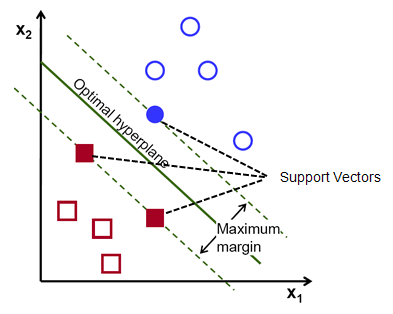
\includegraphics{Pictures/SVM_margin.png}
    \caption{SVM for a linearly classifiable input}
    \label{fig:svm}
\end{figure}
In Figure \ref{fig:svm}, you can see a SVM classifier for a linearly classifiable data \cite{svm}.

Now a days,Support Vector Machine (SVM) classifiers is quite popular in the field of classification,regression analysis and novelty detection  in recent years,  \cite{bishop2006pattern} \cite{xie2008research}.In EEG classifiers, it has been seen that SVM gave very promising results  \cite{lal2004support}. A kernel-based algorithm has been use in Support Vector Machine to give sparse solutions.Support Vector Machine is a computationally efficient method for solving high dimensional  and complex problems, because a  kernel solution required  only for a specific subset of the training data ,not for  the entire training set.  The Support Vector Machine converges to a single minimum and also good in classification of  nonlinear data, and it makes SVM preferable to  neural network or linear  classifiers. A hyper-plane or set of hyper-planes (in a high- or infinite-dimensional space) has been constructed in SVM, which is used for  regression, classification,or other tasks e.g. outliers detection. Intuitively, a hyper-plane is a  good separator of two class.It has the highest length of project to the nearest training-data point of any class.It is also called functional margin.The  margin is inversely proportional to  the generalization error of the classifier  \cite{bishop2006pattern}:

\begin{equation}
    y(x)=w^T\varphi(x)+b 
\end{equation}

\subsection{Decision Tree}
A decision tree a method which is used for regression and classification with no hyper-parameters.It is a supervised learning method.It is a tree like structure, where node denotes feature to be tested and branches can be chose on the basis of that feature value. 

While learning a decision tree,based on a feature value, test we split the source set into subsets.We repeat this process on each derived sub-tree in a recursive manner,this is called recursive partitioning.When the subset at a node have all same value target variable or no value can be added in the prediction by further splitting, we stop the recursion. The construction of DT classifier does not require any  domain specific knowledge or any parameter setting, and therefore for exploratory knowledge discovery, it is appropriated .The higher dimensional data can be utilized while learning a decision trees. In general, we can get a good accuracy with decision tree classifier.


\begin{figure}[ht]
    \centering
    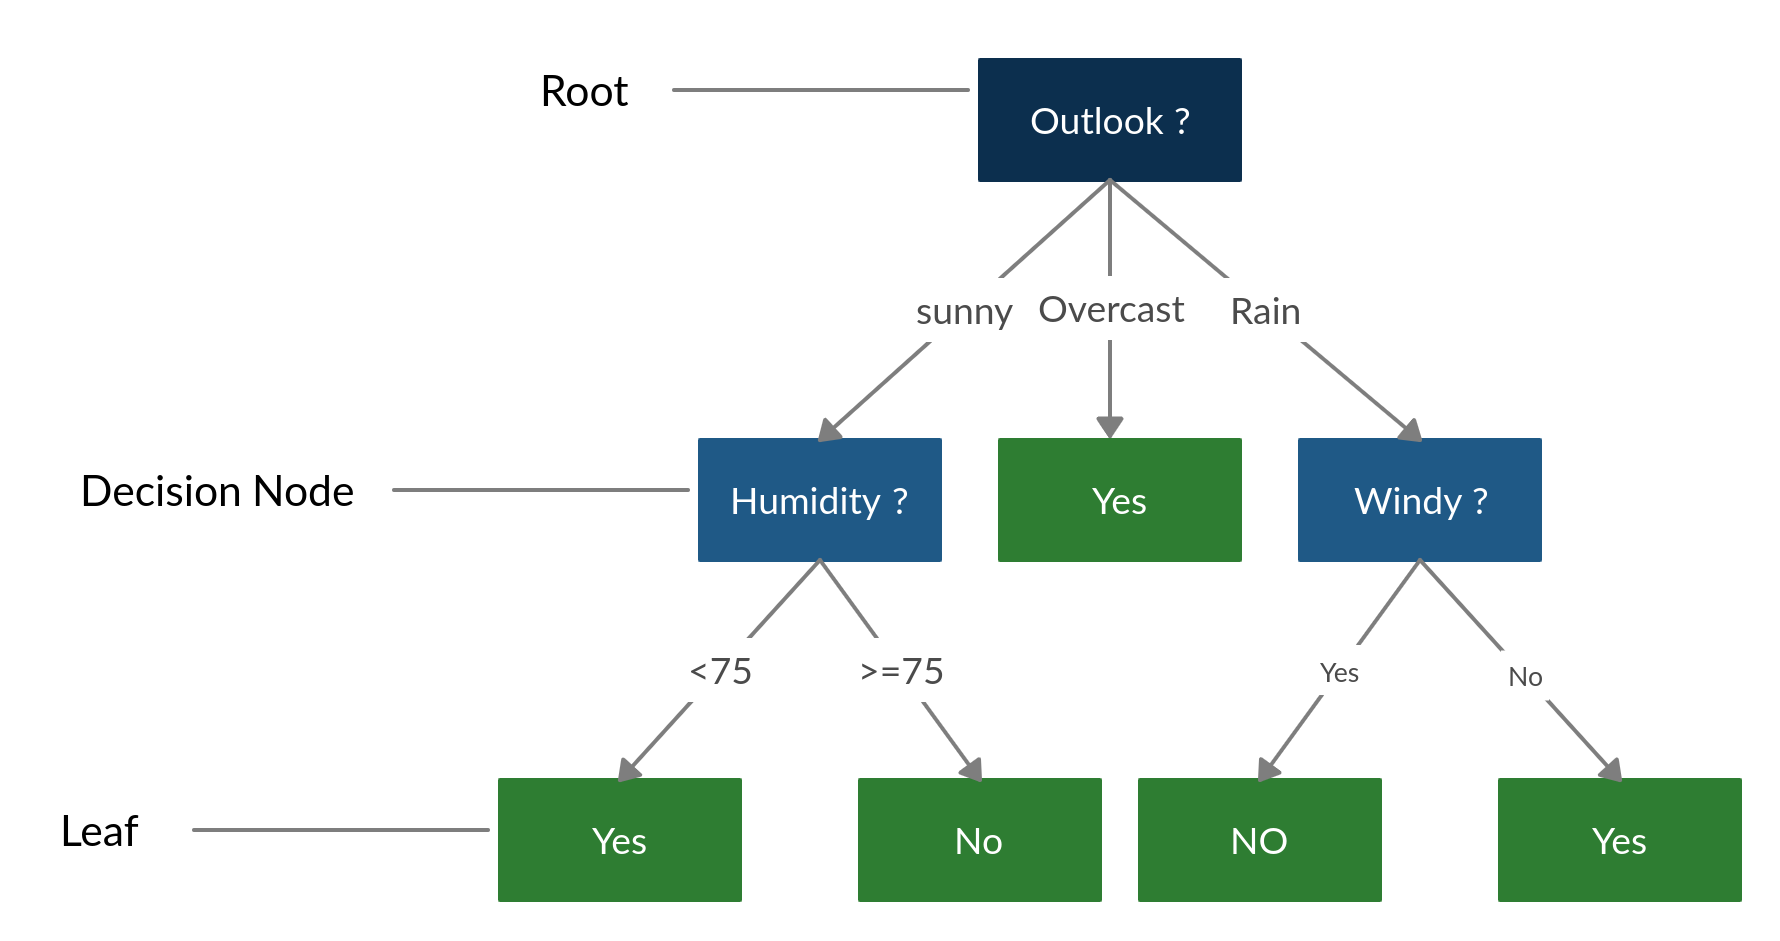
\includegraphics[width=15cm]{Pictures/decision_tres_1.jpg}
    \caption{An example of decision tree.}
    \label{fig:decision_tree}
\end{figure}

The algorithm used to build  DT is called ID3.  J. R. Quinlan developed a top-down, greedy search through the space of possible branches with no backtracking approach has been used in this algorithm . ID3 uses Entropy (equation \ref{entropy} )and Information Gain (equation \ref{gain}) to split a set to subsets,while constructing  a decision tree.
\subsubsection{Entropy} : measure of randomness
\begin{equation}
    E(S)=\sum_{i=1}^c -p_i log_2 p_i
    \label{entropy}
\end{equation}
Here,\\
S:class name\\
c: types of values (2 for binary ) \\
$p_i$ : count of values of $i^{th}$ type\\
\subsubsection{Gain} : gain in entropy after splitting in to subsets
    \begin{equation}
        G(T,X) = E(T) - E(T,X)
        \label{gain}
    \end{equation}
An illustrative example has been shown in Figure \ref{fig:decision_tree}.In the Figure \ref{fig:decision_tree} if the outlook is sunny then we predict on the basis of  humidity,if it is rainy then we check the wind.   
\subsection{Gradient Boosting Classifier}

It is an ML model for classification and regression problems, in which a prediction model has to be constructed in the form of a combination of weak prediction models, typically decision trees used as a week prediction model.Like other boosting methods do gradient boosting algorithm also builds the model in a stage-wise fashion , and to generalize them it allow optimization of an arbitrary differentiable loss function.

% \subsection{Perceptron}

\subsection{XgBoost}
XGBoost is the leading model for working with standard tabular data.To reach peak accuracy, XGBoost models require more knowledge and model tuning than techniques like Random Forest.XGBoost is an implementation of the Gradient Boosted Decision Trees algorithm.Figure \ref{fig:xg_boost} shows a flow diagram of xgBoost.
\begin{figure}
    \centering
    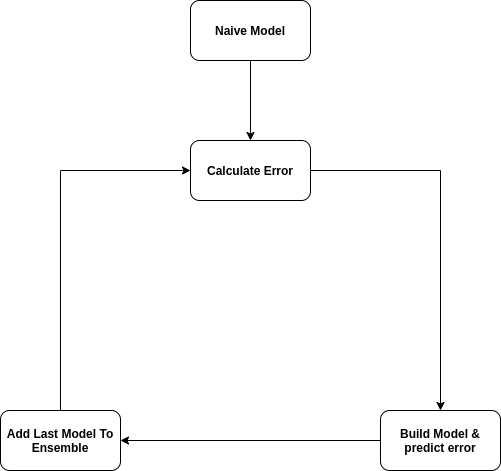
\includegraphics[width=10cm]{Pictures/xgboost.png}
    \caption{XgBoost Flow Chart}
    \label{fig:xg_boost}
\end{figure}

\subsection{Random Forest}
Random forest is a bootstrapping algorithm which uses Decision tree classifier.In our case there is 977 observations with 3328 attribute each.With different initial variables ad different samples, Random forest tries to build multiple decision tree models . For instance, it will build a decision model with a random sample of 100 observation and 5 randomly chosen initial variables. To  make a final prediction, it repeats the process (say) 10 times on every instance. The final prediction is the return of a function which operates on each prediction. We can just take the mean of all the prediction to give final prediction.In Figure \ref{fig:random_forest} we have shown diagram of random forest processing.


\begin{figure}[ht]
    \centering
    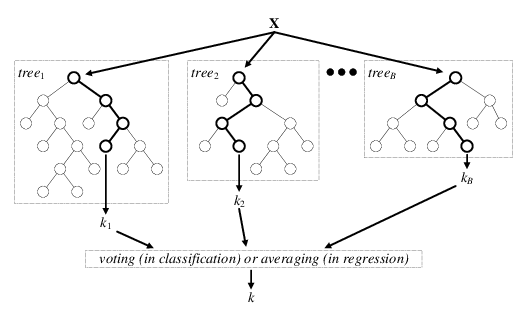
\includegraphics[width=15cm]{Pictures/random_forest_1.png}
    \caption{Random Forest diagram \cite{randomforest} }
    \label{fig:random_forest}
\end{figure}


In the Figure \ref{fig:random_forest},the final prediction will be the value obtained by using voting or averaging method on the predictions of $tree_1$, $tree_2$ ... $tree_B$ i.e. the $k_1,k_2$ and $k_3$.  
% Chapter Template

\chapter{Result} % Main chapter title

\label{Chapter5} % Change X to a consecutive number; for referencing this chapter elsewhere, use \ref{ChapterX}

\lhead{Chapter 5. \emph{Result }} % Change X to a consecutive number; this is for the header on each page - perhaps a shortened title



%----------------------------------------------------------------------------------------
%	SECTION 1
%----------------------------------------------------------------------------------------

\section{Result}
Analysis of the features extracted from the acquired EEG signals of both subjects led to the identification of multiple mind wandering episodes on each session.We have used different classifiers to classify the data and compared their accuracy.The result of different classifiers shown in the below tables.

To understand the result we have know some terms.That are -
\begin{equation}
    f1 score = 2 * \frac{Precision * Recall}{ Precision + Recall }
\end{equation}

\begin{equation}
    Precision = \frac{TP}{FP + TP}
\end{equation}
\begin{equation}
    Accuracy = \frac{TN + TP }{TN+TP+PN+FP}
\end{equation}
\begin{equation}
    Recall = \frac{TP}{ FN + TP}
\end{equation}

Here,\\
FN: False Neagative value \\
TN: True Negative value \\
TP: True positive value \\
FP:False Positive value \\

\subsection{Results of Adaptive boost  :}
we have used decision tree classifier with maximum depth 10 and n\_estimator is equal to 100.Table \ref{tab:adaboost_res} shows the results.
The hyperparameter are sat as follows:\\
maximum depth of decision trees=3,\\
n\_estimators=200\\
\begin{table}[ht]
    \centering
    \caption{Adaptive Boost Result}
    % \begin{center}
    {\renewcommand{\arraystretch}{1.2}
    \begin{tabular}{ccccc}
            \hline
            \hline
             & Precision & Recall & F1 Score & Support \\ 
            \hline
              Alertness   & 0.88 & 0.89 & 0.89 & 114  \\
              Mind Wandering   & 0.85 & 0.84 & 0.85 & 82 \\
              accuracy &  &  & 0.87 & 196 \\
              \hline
              \hline
        \end{tabular}
    }
    % \end{center}
    
    \label{tab:adaboost_res}
\end{table}

\subsection{Results of Decision tree}
For the accuracy and other training details see Table \ref{tab:decison_tree_res}.
\begin{center}
    \begin{table}[ht]
    \centering
    \caption{Results of Decision Tree Testing}
    {\renewcommand{\arraystretch}{1.2}
    \begin{tabular}{ccccc}
       \hline
       \hline
         & Precision & Recall & F1 Score & Support \\
        \hline
          
         Alertness      & 0.81   &   0.91     & 0.86     &  114 \\
         Mind Wandering      & 0.85   &   0.70     & 0.77      &  82 \\
    accuracy      &        &           & 0.82     &  196 \\
 
          \hline
          \hline
    \end{tabular}
    }
    \label{tab:decison_tree_res}
\end{table}
\end{center}


\subsection{Results of Gradient Boosting classifier }
Table \ref{tab:Gradient_Boosting_classifier_res} shows the data obtained during testing trained Gradient Boosting classifier .
\begin{table}[ht]
    \centering
    \caption{Results of Gradient Boosting classifier }
    {\renewcommand{\arraystretch}{1.2}
    \begin{tabular}{ccccc}
       \hline
       \hline
         & Precision & Recall & F1 Score & Support \\
        \hline
        
         Alertness      & 0.88     & 0.85     & 0.87       &114 \\
         Mind Wandering      & 0.80     & 0.84     & 0.82        &82 \\
    accuracy      &         &           & 0.85       &196 \\
          \hline
          \hline
    \end{tabular}
    }
    \label{tab:Gradient_Boosting_classifier_res}
\end{table}

\subsection{Results of Random Forest }
You can see the accuracy,precision and recall of Random Forest Classifier in Table \ref{tab:rf_res}.The highest accuracy measured at n\_estimator=102. 
\begin{table}[ht]
    \centering
    \caption{Results of Random Forest classifier }
    {\renewcommand{\arraystretch}{1.2}
    \begin{tabular}{ccccc}
       \hline
       \hline
         & Precision & Recall & F1 Score & Support \\
        \hline
          Alertness &      0.88     & 0.90  &    0.89      & 114 \\
         Mind Wandering    &   0.86     & 0.83     & 0.84       & 82 \\
    accuracy    &           &           & 0.87      & 196 \\
          \hline
          \hline
    \end{tabular}
    }
    \label{tab:rf_res}
\end{table}

\subsection{Results of XgBoost }
In Table \ref{fig:xg_boost}, we have listed the accuracy, precision,recall and f1-score for mind wandering and alertness state.  
\begin{table}[ht]
    \centering
     \caption{Results of xgBoost classifier }
     {\renewcommand{\arraystretch}{1.2}
    \begin{tabular}{ccccc}
       \hline
       \hline
         & Precision & Recall & F1 Score & Support \\
        \hline
          Alertness   &    0.88    &  0.88      & 0.88      & 114 \\
         Mind Wandering      & 0.83 &     0.84      & 0.84       & 82 \\
    accuracy   &            &            & 0.86      & 196 \\
          \hline
          \hline
    \end{tabular}
    }
    \label{tab:xqboost_res}
\end{table}

\subsection{Results of Support Vector Machine }
The optimal accuracy we got when hyper-parameters sat as shown below:\\
kernel: rbf,\\
gamma: scale,\\
C:6 \\ 
and the results are shown in Table \ref{tab:SVM_res}.
\begin{table}[ht]
    \centering
    \caption{Results of SVM classifier}
    {\renewcommand{\arraystretch}{1.2}
    \begin{tabular}{ccccc}
       \hline
       \hline
         & Precision & Recall & F1 Score & Support \\
        \hline
         Alertness    &   0.83 &    0.93 &     0.88 &       114\\
         Mind Wandering    &   0.88  &    0.73 &      0.80      &  82 \\
        accuracy    &          &            &     0.85      & 196 \\
          \hline
          \hline
    \end{tabular}
    }
    \label{tab:SVM_res}
\end{table}
%-----------------------------------
%	SUBSECTION 1
%-----------------------------------
 
% Chapter Template

\chapter{Discussion} % Main chapter title

\label{Chapter6} % Change X to a consecutive number; for referencing this chapter elsewhere, use \ref{ChapterX}

\lhead{Chapter 6. \emph{Discussion}} % Change X to a consecutive number; this is for the header on each page - perhaps a shortened title

%----------------------------------------------------------------------------------------
%	SECTION 1
%----------------------------------------------------------------------------------------
% \section{Discussion}

We have analysed the EEG signals from 64 channels to detect the mind wandering state using some basic machine learning techniques.After trying 6 machine learning classifiers, we are able to detect MW and Alertness state with 87\% accuracy.By analysing the test results from all six classifiers, we observed a pattern that is the precision and recall of  Alertness state detection is higher than  Mind Wandering state.So, we can say that we are able to predict Alertness more precisely than MW.And similarly you can see  that F1-score for MW is lower than Alertness (Figure \ref{fig:test_score}).And you can also see different comparison in the Figure \ref{fig:test_score}.


\begin{figure}
    \subfigure[]{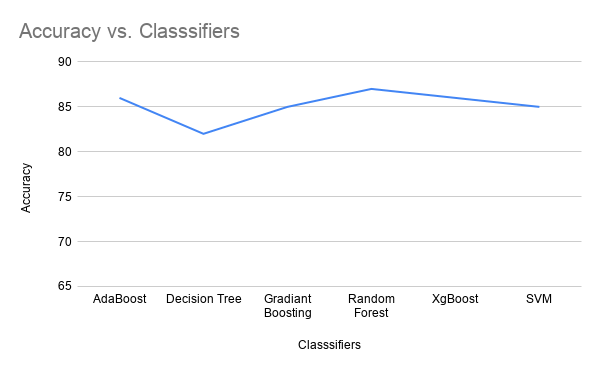
\includegraphics[width=0.49\textwidth]{Pictures/Accuracy vs. Classsifiers (1).png}}
    \subfigure[]{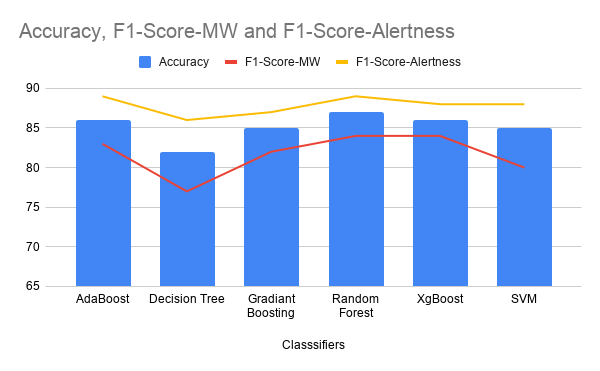
\includegraphics[width=0.49\textwidth]{Pictures/Accuracy, F1-Score-MW and F1-Score-Alertness.png}}
    \subfigure[]{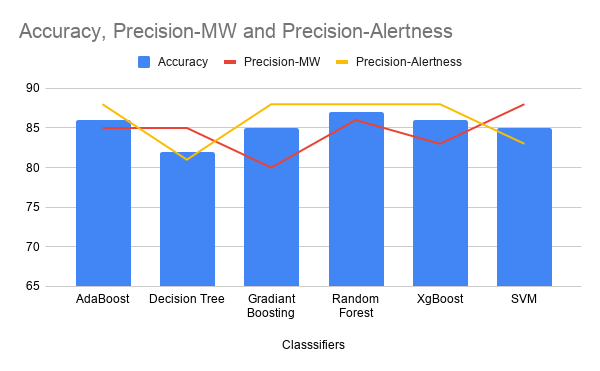
\includegraphics[width=0.49\textwidth]{Pictures/Accuracy, Precision-MW and Precision-Alertness.png}}
    \subfigure[]{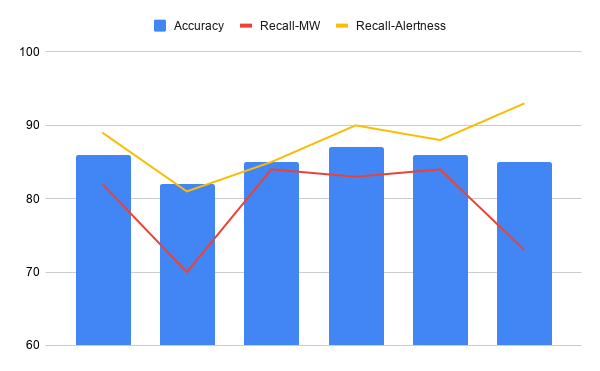
\includegraphics[width=0.49\textwidth]{Pictures/chart (1).png}}
    
    \subfigure[]{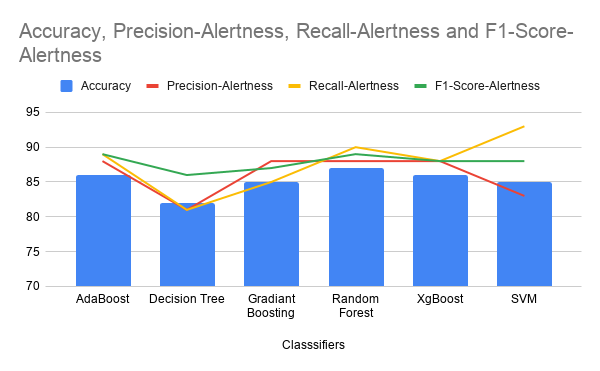
\includegraphics[width=0.49\textwidth]{Pictures/Accuracy, Precision-Alertness, Recall-Alertness and F1-Score-Alertness (1).png}}
    \subfigure[]{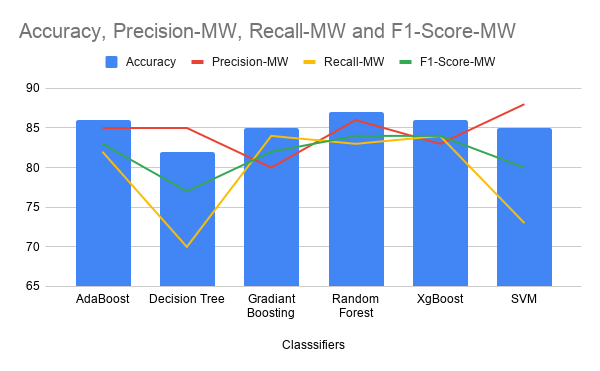
\includegraphics[width=0.49\textwidth]{Pictures/Accuracy, Precision-MW, Recall-MW and F1-Score-MW.png}}
    \centering
    % 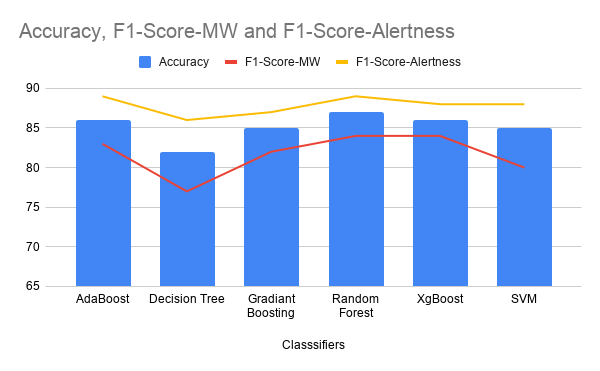
\includegraphics[width=10cm]{Pictures/Accuracy, F1-Score-MW and F1-Score-Alertness.png}
    \caption{Classifier results,bar chart is for accuracy and line chart is for precision,recall and F1-score (a) accuracy vs classifier, (b) comparison of F1-score  for MW and Alertness for different classifier, (c) comparison of precision  for MW and Alertness for different classifier, and (d) comparison of recall  for MW and Alertness for different classifier,  (e) comparison of recall,f1-score and precision for alertness for different classifier, and (f)  comparison of recall,f1-score and precision for MW for different classifier,  }
    \label{fig:test_score}
\end{figure}


The highest accuracy, that we got by analysing EEG-signals from 64 channels using 6 different basic machine learning  classifiers is 87\% which is higher than any research have been done in this area.We have got the highest accuracy on Random Forest classifier.Before applying classifier we extracted MW \& alertness data from continuous channel signals, normalized them,extracted feature set for all 64 channels of size 52 and flattened them by concatenating each channel data.Then we have applied classifiers.By comparing all the results we can safely deduce that by using XgBoost,Random Forest and Ada-Boost ML classifiers to detect MW and alertness state with a 86-87 \% accuracy.
% Chapter Template

\chapter{Conclusion} % Main chapter title

\label{Chapter7} % Change X to a consecutive number; for referencing this chapter elsewhere, use \ref{ChapterX}

\lhead{Chapter 7. \emph{Conclusion}} % Change X to a consecutive number; this is for the header on each page - perhaps a shortened title

%----------------------------------------------------------------------------------------
%	SECTION 1
%----------------------------------------------------------------------------------------
Now a days,there are many new inventions are happening day by day.Each invention added new comfort to the human life.And, people are also excited for new innovative technologies which provides a little comfort, mind wandering getting predicted  (MW), its effects on emotion are getting studied , in the near future the consequence it brings will be playing a fundamental role . In on our approach we predicted MW with 87\% accuracy with random forest classifier.Different classification techniques were used to predict MW episodes and Alertness periods by putting the values on different algorithms for a better accuracy.The  random forest classifier seems very handy on extracted features as it is accurate on processing EEG data. It can also be observed that the features such as wavelet parameters,Skewness,Kurtosis,first \& second differences,mean,coefficient of variable etc. cumulatively have provided better classification accuracy. We would like to measure physical activities in real-time using our proposed approach and utilize this concept in various places as per need in the future.In real time application(such as driver ,security person attention detection,student attentiveness in the class etc.),to detect if a person is alert or not,the result obtained in this study may be quite help full.There are some studies on the same topic with Deep Learning ( in general Deep Learning give better accuracy than Machine learning),but the accuracy that we have measured is the comparable to them. There are few researches on this and more coming up with more interesting aspects of MW and soon it is predicted to be one of the largely growing topics to work on

%----------------------------------------------------------------------------------------
%	THESIS CONTENT - APPENDICES
%----------------------------------------------------------------------------------------

\addtocontents{toc}{\vspace{2em}} % Add a gap in the Contents, for aesthetics

% \appendix % Cue to tell LaTeX that the following 'chapters' are Appendices

% Include the appendices of the thesis as separate files from the Appendices folder
% Uncomment the lines as you write the Appendices

% Appendix Template

% \chapter{Appendix A} % Main appendix title

% \label{AppendixX} % Change X to a consecutive letter; for referencing this appendix elsewhere, use \ref{AppendixX}

% \lhead{Appendix X. \emph{Appendix Title Here}} % Change X to a consecutive letter; this is for the header on each page - perhaps a shortened title



% \input{Appendices/AppendixB}
%\input{Appendices/AppendixC}

\addtocontents{toc}{} % Add a gap in the Contents, for aesthetics

\backmatter


%----------------------------------------------------------------------------------------
%	BIBLIOGRAPHY
%----------------------------------------------------------------------------------------
% \nocite{*}
\label{Bibliography}

\lhead{\emph{Bibliography}} % Change the page header to say "Bibliography"

\bibliographystyle{apalike} % Use the "custom" BibTeX style for formatting the Bibliography

\bibliography{Bibliography} % The references (bibliography) information are stored in the file named "Bibliography.bib"
% \begin{enumerate}
%     \item Michael D. Greicius , Ben Krasnow, Allan L. Reiss, and Vinod Menon  "Functional connectivity in the resting brain:A network analysis of the default mode hypothesis" 2002
%     \item https://commons.wikimedia.org/wiki
%     \item Romain Grandchamp 1,2 *, Claire Braboszcz 1,2 and Arnaud Delorme "Oculometric variations during mind wandering"
%     \item P. Fransson and G. Marrelec, ”The precuneus/posterior cingulate cortex plays a pivotal role in the default mode network: Evidence from a partial correlation network analysis,” NeuroImage, vol. 42, no.3, pp. 1178-1184, 2008.
%     \item  A. Vanhaudenhuyse, A. Demertzi, M. Schabus, Q. Noirhomme, S. Bredart, M. Boly, C. Phillips, A. Soddu, A. Luxen, G. Moonen, and S. Laureys, ”Two distinct neuronal networks mediate the awareness of environment and of self.,” Journal of Cognitive Neuroscience, vol.23, no. 3, pp. 570-578, 2011.
%     \item N. C. Andreasen, D. S. O’Leary, T. Cizadlo, S. Arndt, K. Rezai, G.L. Watkins, L. L. B. Ponto, and R. D. Hichwa, ”Remembering the past: Two facets of episodic memory explored with positron emission tomography,” American Journal of Psychiatry, vol. 152, no. 11, pp. 1576-1585, 1995.
%     \item A. M. Dale, A. K. Liu, B. R. Fischl, R. L. Buckner, J. W. Belliveau, J. D. Lewine, and E. Halgren, ”Dynamic Statistical Parametric Mapping,” Neuron, vol. 26, no. 1. pp. 55-67, 2000.
%     \item M. J. Brookes, M. Woolrich, H. Luckhoo, D. Price, J. R. Hale, M.C. Stephenson, G. R. Barnes, S. M. Smith, and P. G. Morris, ”Investigating the electrophysiological basis of resting state networks using magnetoencephalography.,” Proceedings of the National Academy of Sciences of the United States of America, vol. 108, no. 40, pp. 16783-8, Oct. 2011.
%     \item S. Whitfield-Gabrieli and J. M. Ford, ”Default Mode Network Activity and Connectivity in Psychopathology,” Annual Review of Clinical Psychology, vol. 8, no. 1. pp. 49-76, 2012.
% \end{enumerate}
\end{document}  
